\documentclass[]{article}
\usepackage[utf8]{inputenc}
\usepackage{graphicx}
\usepackage{float}
\usepackage{amssymb}
%\usepackage{amsmath}
\usepackage{setspace}
\usepackage[top=1in, bottom=1in, left=1in, right=1in]{geometry}
\usepackage{fancyhdr}
\usepackage{multicol}
\usepackage{wrapfig}
\usepackage{todonotes}
\usepackage{syntonly} 
%\syntaxonly

\title{E158 - VLSI Final Project: Tic-Tac-Toe}
\author{Katherine Yang and Guillaume Legrain}
\date{April 2015}

\begin{document}
%% Cover page
%• Project title, designers, and a chip plot
\maketitle
{\centering
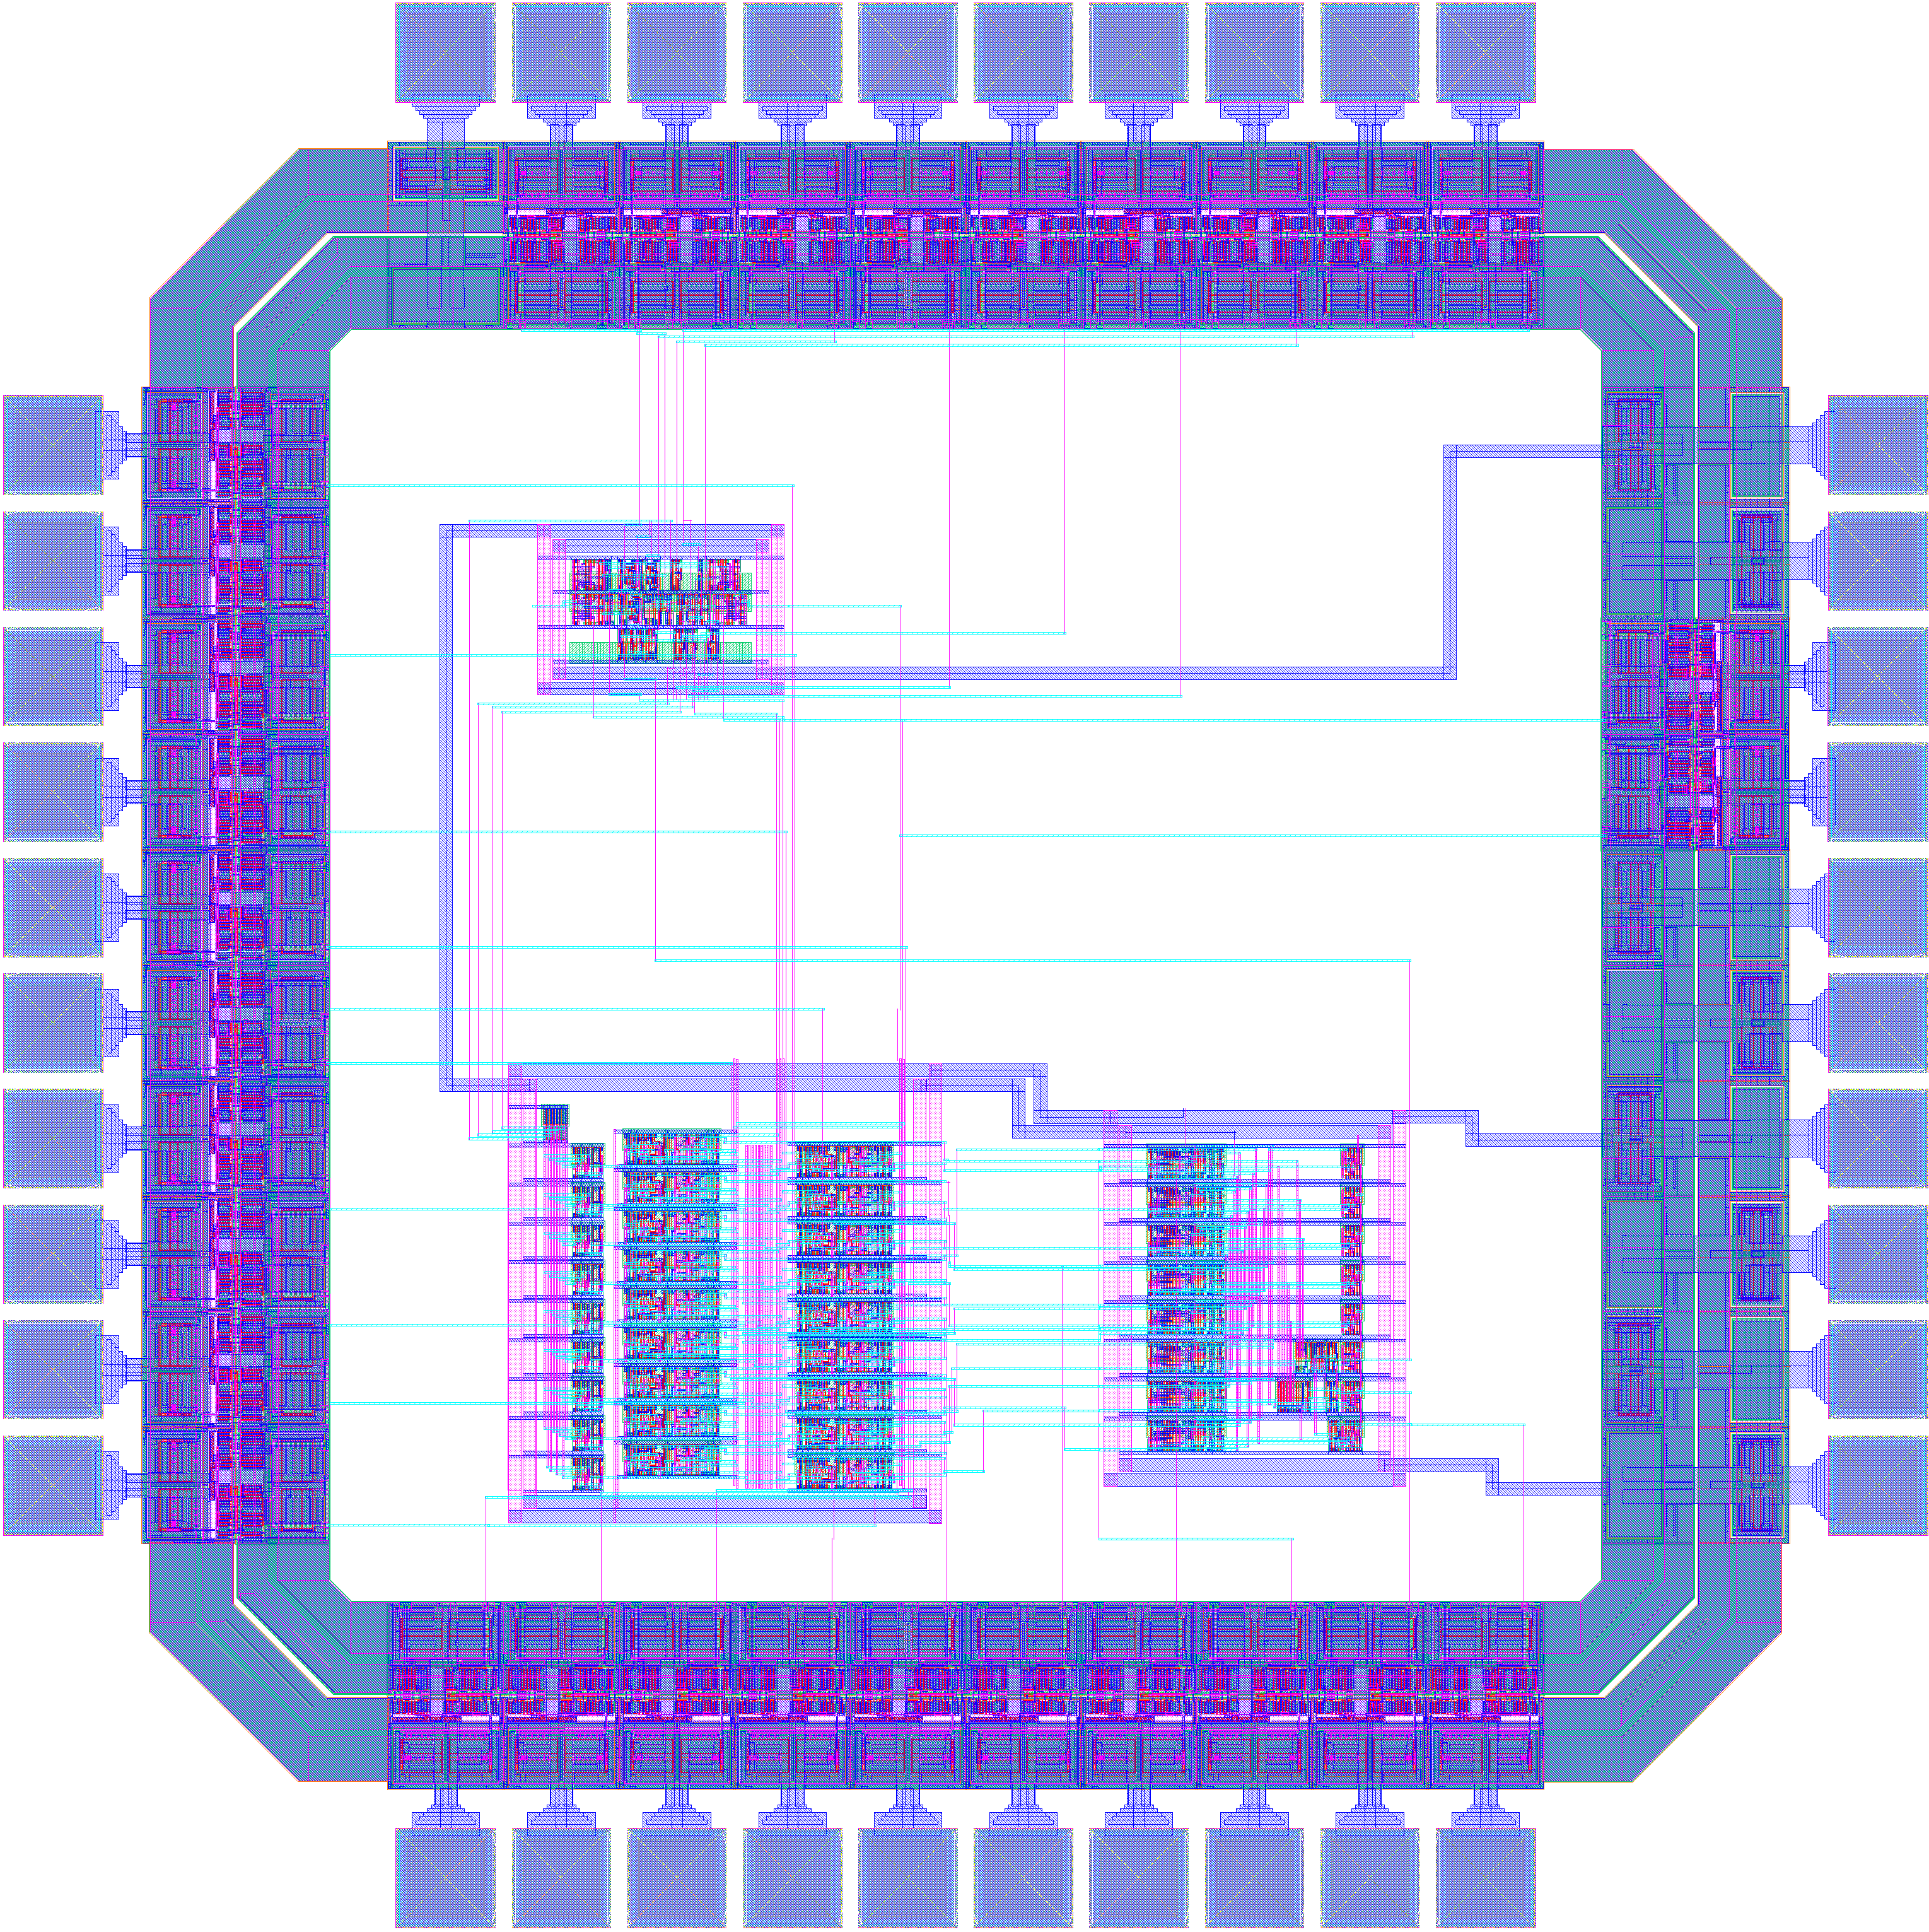
\includegraphics[scale=0.15]{chip-layout} \par
}

\clearpage

%%%%%%%%%%%%%%%%%%%%%%%%%
%  Introduction
%%%%%%%%%%%%%%%%%%%%%%%%%
\section{Introduction}
\label{sec:introduction}
% A brief high-level description of the chip function and the manufacturing process
This project is a 3x3 game of Tic-tac-toe built on a $0.6~\mu m$ process on a $1.5 \times 1.5~mm$ 40-pin MOSIS ``TinyChip''. The goal of this project is to create a Tic-Tac-Toe board which is able to monitor the state of a game and return the win/lose/draw state of the game after each player's move. Specifically, for each player's turn, the game records the player's inputs and at the end of the game determines if the game is done and who the winner is. The game allows two players to play against each other. Each of the nine spaces can be ``X'', ``O'' or blank. 


\section{Specifications}
\label{specifications}
% Table of inputs, outputs indicating name, direction, bus widths
% Theory of operation of the chip relating the outputs to the inputs
The chip will have a total of 32 I/O pins plus 4 GND pins and 4 VDD pins.
User input is a 4-bit vector (\texttt{playerInput<3:0>}) to describe the cell number at which to play. The write input will signal the game controller that the playerInput is ready to read/write. \texttt{gameState<1:0>} is used to represent the state of the game: player 1's turn, player 2's turn or end. As the name implies \texttt{winner<1:0>} describes who won the game: player 1, player 2, tie when the game is not done. To prevent hold time issues, the system will be using two non-overlapping clocks. Thus, the chip uses a two-phase clock with pins \texttt{ph1} and \texttt{ph2}. A list of all inputs can be found in table~\ref{tab:io-list}.


\begin{table}
\centering
\caption{List of I/O pins for a total of 32 pins}
\begin{tabular}{ | l | l | l | p{5cm} |}
\hline
    Function (\emph{Name})               & I/O type     & Bus Width & Description \\
\hline
    Power (\emph {vdd})                  & Input/Output & 1         & Provides power \\
\hline
    Ground (\emph{gnd})                  & Input/Output & 1         & Ground \\
\hline
    Reset (\emph{reset})                 & Input        & 1         & Resets the board to empty \\
\hline 
    Clock (\emph{ph1, ph2})              & Input        & 2         & Two phase clock\\
\hline
    First Player (\emph{isPlayer1Start}) & Input        & 1         & Determines which player plays "X" or "O" \\
\hline
    Write Confirmation (\emph{playerWrite}) & Input     & 1         & Confirms the current player input \\
\hline
    Input Position (\emph{playerInput})    & Input      & 4         & Indicates which position on the game board the player played \\
\hline
    Game Complete (\emph{gameIsDone})      & Output     & 1         & Determines if game is complete \\
\hline
    Winner (\emph{winner}) & Output & 2 & Displays \texttt{11} if player 1 wins, \texttt{10} if player 2 wins, and \texttt{01} if there is a draw \\
\hline
    Game State (\emph{gameState}) & Output              & 3         & Indicates which player's turn it is to play or if the game is done\\
\hline
    Game Board (\emph{gBoard})              & Output     & 18        & Displays the current state of the game \\
    \hline
\end{tabular}

\label{tab:io-list}
\end{table}


%%%%%%%%%%%%%%%%%%%%%%%%%
%  Floorplan
%%%%%%%%%%%%%%%%%%%%%%%%%
\section{Floorplan}
\label{sec:floorplan}
% • Compare the actual floorplan to the proposal and explain discrepancies\\
% • Slice plan for datapath(s)\\
% • Pinout diagram indicating names and pin numbers for each pin
Figure~\ref{fig:floorplan} shows the chip floorplan for  the tic-tac-toe chip including the pad frame. The top-level blocks are the game controller, the datapath and the memory. A wiring channel is located between the controllers and datapath and between the datapah and memory to provide room to route control signals to the datapath. The \emph{pad frame} includes 40 I/O pads, which are wired to the pins on the chip package. As listed in table~\ref{tab:io-list}, there are 32 pads used for signal; the remainder are $V_{DD}$ and GND. Figure ~\ref{fig.pinout} shows the pinout diagram indicating names and pin numbers for each pin.

\begin{figure}
\centering
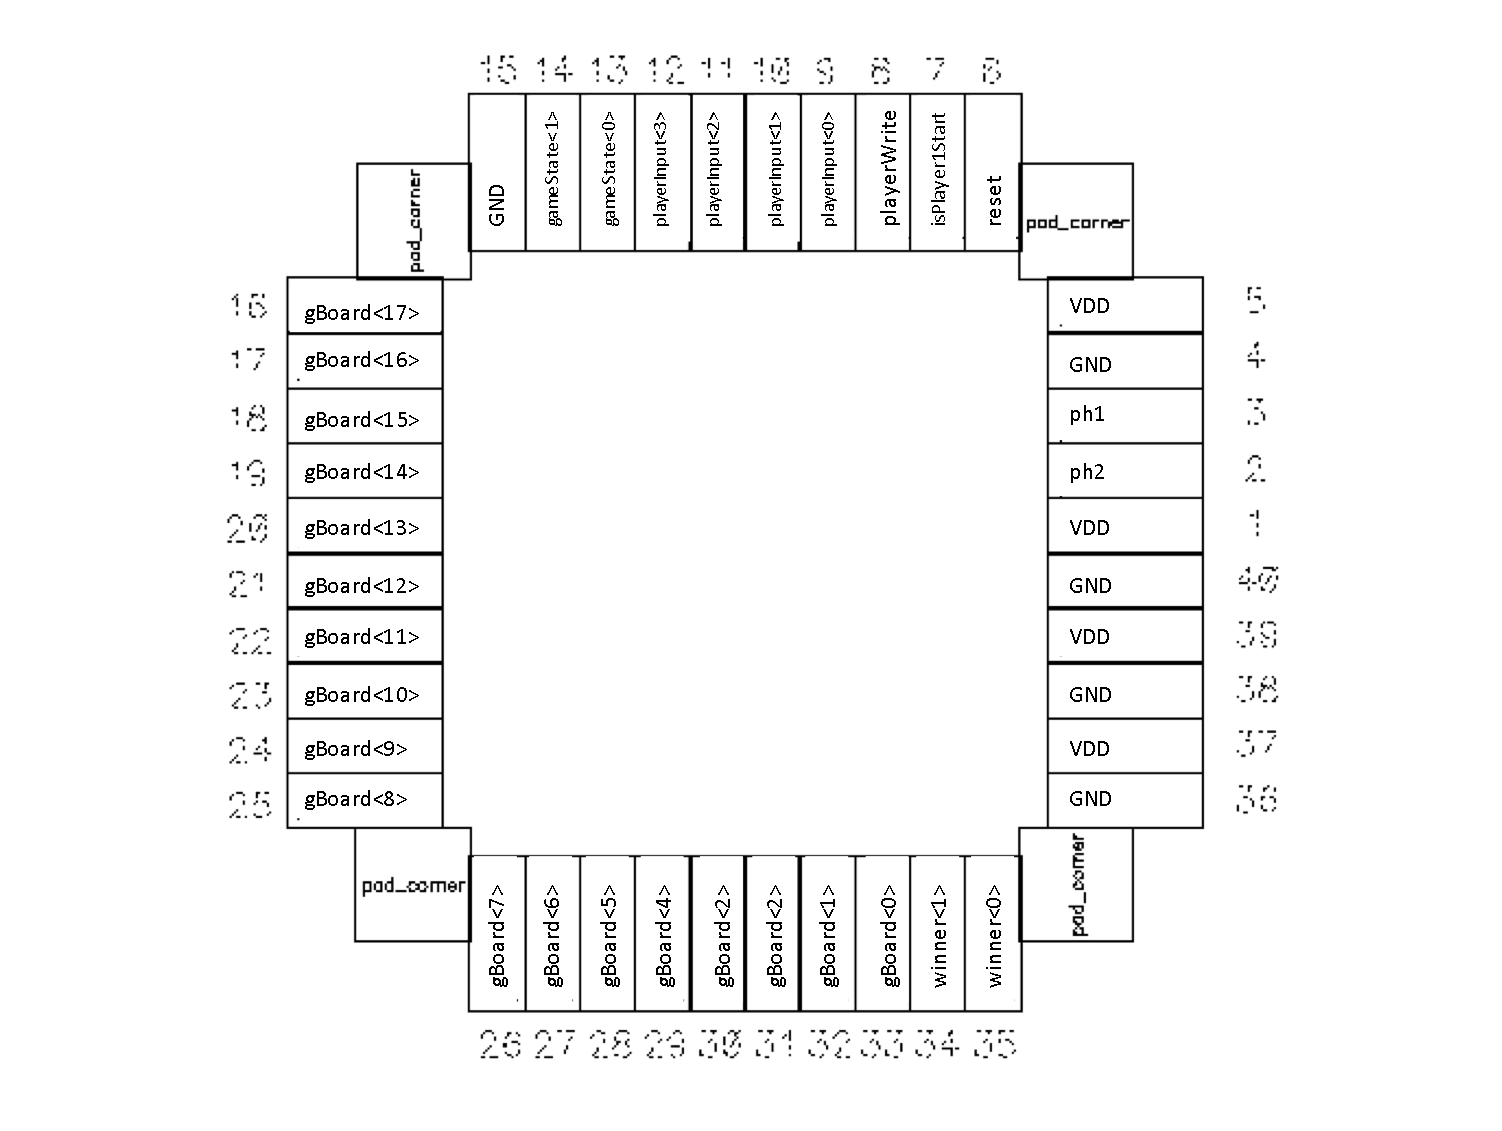
\includegraphics[width=.2\textwidth]{pinout}
\caption{Tic-tac-toe pinout diagram}
\label{fig:pinout}
\end{figure}

The floorplan is drawn to estimated scale size in fig.~\ref{fig:floorplan}. The chip is designed in a $0.6~\mu m$ process on 1.5x1.5 mm die so the die is $5000~\lambda$
on a side. Each pad is $750 \lambda \times 350 \lambda$
\cite{e85-book}.


\begin{figure}
\centering
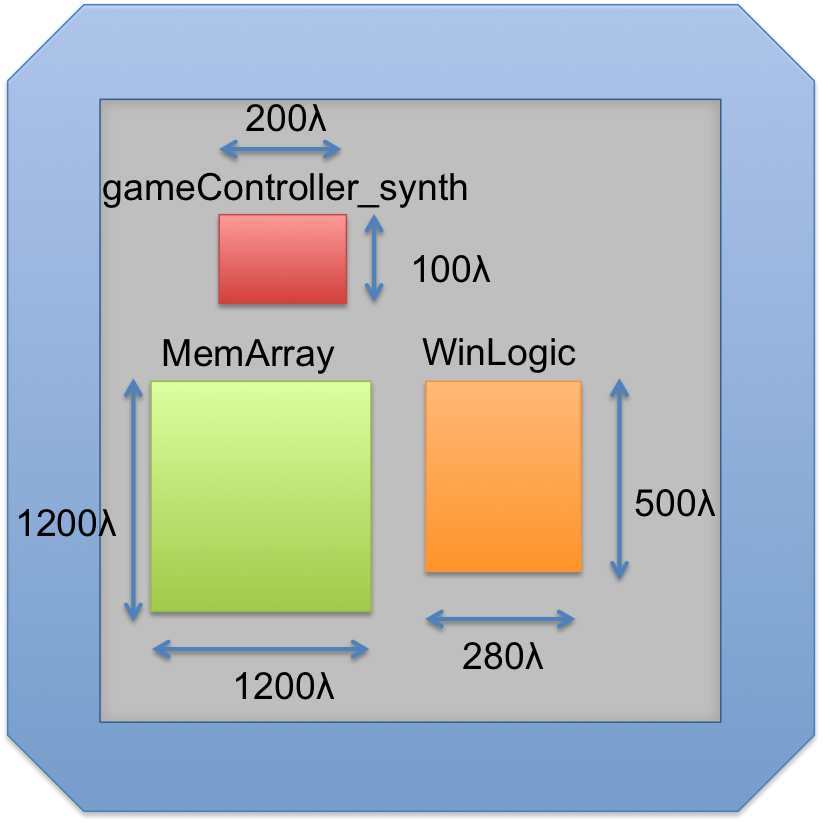
\includegraphics[width=.2\textwidth]{chipsize}
\caption{Tic-tac-toe floorplan}
\label{fig:floorplan}
\end{figure}

\subsection{Top Level Blocks}
\subsection{Synthesized Blocks}
\begin{itemize}
\item Game controller FSM
\item ``AI'' FSM
\end{itemize}

\subsection{Custom Blocks}
\begin{itemize}
\item Memory array with decoder logic
 \item datapath: win logic
 \end{itemize}

\section{Slice Plans}
Both the memory array and the win logic will be laid out with 8 words of 2-bit length.

% \clearpage
% \onecolumn


%%%%%%%%%%%%%%%%%%%%%%%%%
%  Verification
%%%%%%%%%%%%%%%%%%%%%%%%%
\section{Verification}
\label{sec:verification}

All Verilog code successfully simulates using their respective testbenches and sets of testvectors. All schematics were also successfully tested against the same testbenches.

Every layout component of the system passed DRC and LVS. The exported GDS chip passes DRC with 144 errors related to optional rule 10.4 about spacing from the pad to unrelated metal. 

If the chip was to be fabricated

• Does layout pass DRC and LVS?\\
• Does CIF load correctly and pass DRC and LVS?\\
• If the chip contains any analog blocks, show the HSPICE simulations\\
• Explain any discrepancies or concerns\\
• Postfabrication test plan\\
• How will the chip be tested if it is fabricated?

%%%%%%%%%%%%%%%%%%%%%%%%%
%  Summary
%%%%%%%%%%%%%%%%%%%%%%%%%
\section{Summary}
\label{sec:summary}


%%%%%%%%%%%%%%%%%%%%%%%%%
%  Desgin Time
%%%%%%%%%%%%%%%%%%%%%%%%%
\subsection{Design Time}
\label{sec:designtime}
A summary of design time spent on each component of the project is shown in table ~\ref{tab:designtime}

\begin{table}
\centering
\caption{Table of design time for each component}
\begin{tabular}{ | l | l | l |}
\hline
    Component             & Time Spent (hrs) \\
\hline
    Project Proposal        & ~7 \\
\hline
    Verilog                 & ~30\\
\hline
    Schematic               & ~20\\
\hline
    Layout                  & ~40\\
\hline
    \textbf{Total Time spent:}& \textbf{~97} \\
\hline
\end{tabular}

\label{tab:designtime}
\end{table}
\subsection{File Locations}
\label{sec:filelocations}
\begin{table}
\centering
\caption{File locations for each component}
\begin{tabular}{ |p{3cm} | l |}
\hline
    Item                & Location \\
\hline
    Verilog testbench   & https://github.com/glegrain/Tic-tac-toe\\
\hline
    Testvectors         & https://github.com/glegrain/Tic-tac-toe\\
\hline
    Synthesis Results   & /home/glegrain/IC\_CAD/cadence/texttt{*.rep, *pow}\\
\hline
    GDS                 & /home/glegrain/IC\_CAD/cadence/chip.gds\\
\hline
    Cadence Libraries   & /home/glegrain/IC\_CAD/cadence\\
\hline
    PDF of chip plot    &\\ 
\hline
    Final Report        & \\
\hline  
\end{tabular}

\label{tab:filelocations}
\end{table}
\section{References}
\section{Appendices}
• Verilog code and testbench (in monospaced font such as Courier 8 pt, with columns lining up and lines wrapping cleanly)\\
• Include test vectors unless they are unreasonably long\\
• HSPICE testbench(es), if applicable\\
• Legible schematics of the cells you produced (labeled with cell name)\\
• Do not include large synthesized blocks that are unintelligible\\
• Do not include muddlib cells\\
• Color layouts (labeled with cell name)\\
• Other materials generated during the project 








%%%%%%%%%%%%%%%%%%%%%%%%%
%  Architecture
%%%%%%%%%%%%%%%%%%%%%%%%%
\section{Architecture}
The architecture consists of 3 main modules, one of which will be synthesized, and two will be hand laid.

\subsection{List of modules}
\subsubsection{Memory Array}
The memory array remembers the status of the tic-tac-toe game board through sequential logic. It consists of enable reset flip-flops and a 4 to 8 bit decoder.
\subsubsection{Check Win Status}
The win status module is a combinational logic block that checks the win state of the tic-tac-toe board. There are two custom made leaf cells in this module. This cell is very repetitive and can be organised as a datapath.
\subsubsection{Game Controller}
The game controller module is a finite state machine which switches between players, player input and game board. This module will be synthesized as the structure is more irregular and harder to be hand laid.

\subsection{Game representation}
The Tic-tac-toe game board is represented by 8 cells. Each cell is either empty, a cross or a circle using 2-bits as shown in fig.~\ref{fig:cell-representation}. Thus, the game board is represented by an array of 18-bits as shown in fig.~\ref{fig:gBoard-representation}.

\begin{figure}
\centering
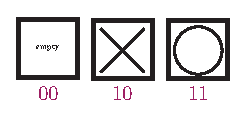
\includegraphics[width=0.2\textwidth]{cell-representation}
\caption{Each cell of the game board is represented using two bits. The MSB is used to describe if the cell has been played or not. The LSB is used to describe who played in the cell.}
\label{fig:cell-representation}
\end{figure}

\begin{figure}
\centering
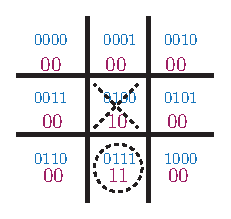
\includegraphics[width=0.2\textwidth]{gBoard-representation}
\caption{The playable game board is represented by 18-bits. Each pair of bits are used to describe a cell. Each cell holds a two bit value and is accessed with a 4-bit address.}
\label{fig:gBoard-representation}
\end{figure}



%%%%%%%%%%%%%%%%%%%%%%%%%
%  Logic design
%%%%%%%%%%%%%%%%%%%%%%%%%
\section{Logic Design}
A top level diagram in fig.~\ref{fig:top-level} show the different blocks of the architecture.

\begin{figure}
\centering
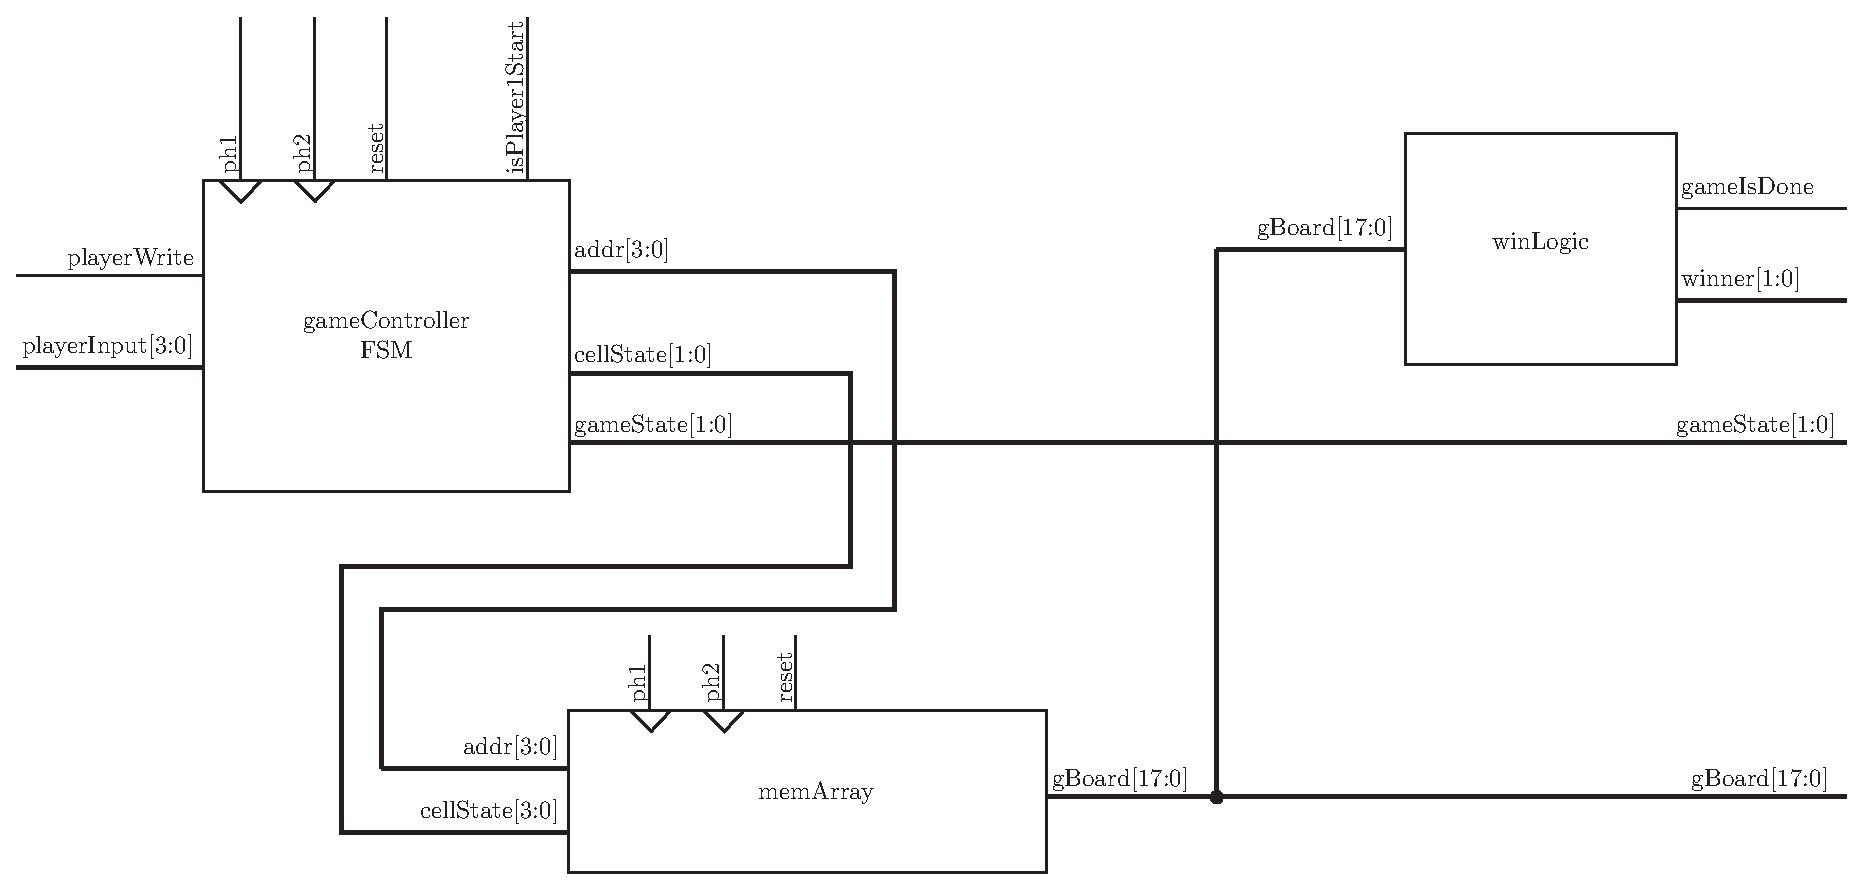
\includegraphics[width=0.8\textwidth]{top-level}
\caption{Top Level Block Diagram of the Tic-tac-toe architecture.}
\label{fig:top-level}
\end{figure}
The blocks are described in each of the sections below. The game controller is in charge of controlling which player is writing to the game board. Player 1 and player 2 enters the address they want to play at, which updates to the memory FF block when it is their respective turn and a write switch is activated. The datapath uses combinational logic determine the winning/losing status of the players.

\subsection{Memory Array}
The \emph{Memory array} is an array of 18-bit flip-flops (9 words of 2-bits) to store the state of the game board. The memory array incorporates a row decoder using the address (\texttt{addr[3:0]} to activate one of the rows by asserting the wordline (\texttt{cellState[1:0]}). The decoder logic for the memory can be seen in figure~\ref{fig:memArray}.

The decoder logic will be using an estimate of 4 cells per ``write'' to enable each pairs of flip-flop. Thus, the decoder logic will be using an estimate of $4\times 9$ logic gates which rounds to a rough size estimate of  $ 1000\lambda \times 188 \lambda$. The flip-flop array height estimate is $18 \times 100\lambda = 1800\lambda$ and the width is $300\lambda$ wide . The total size estimate for the memory block rounded up to $2000 \lambda \times 600 \lambda$.
\begin{figure}
\centering
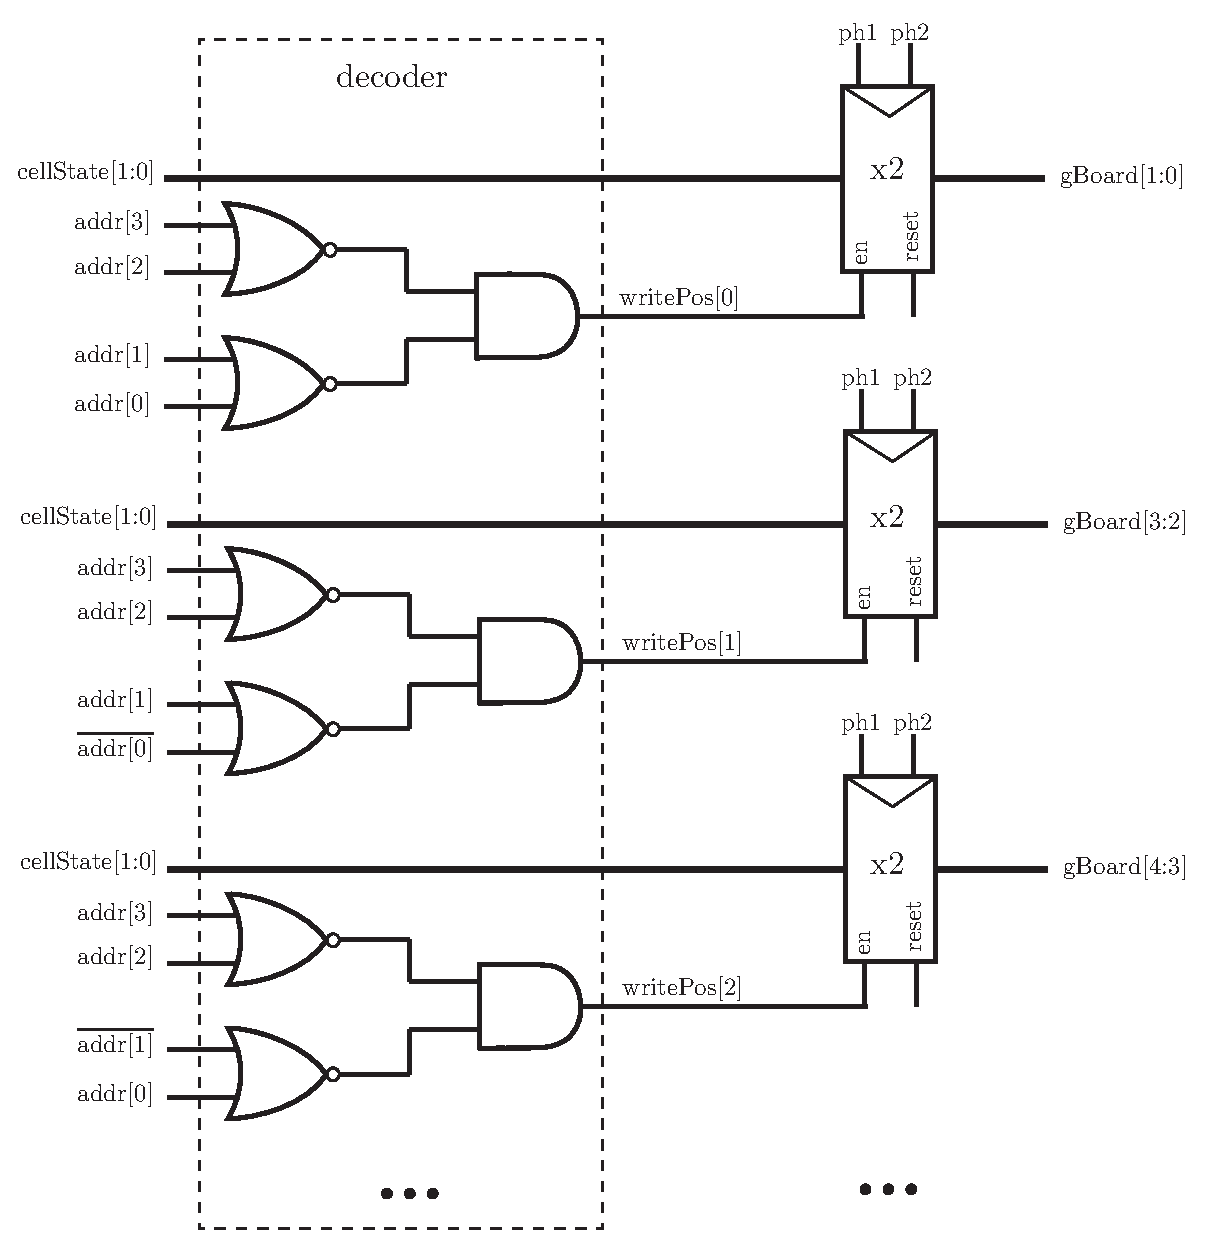
\includegraphics[width=.45\textwidth]{memArray}
\caption{Memory array block made from 18 D-Flip-flops.The row decoder uses the address (\texttt{addr[3:0]} to activate one of the rows by asserting the wordline (\texttt{cellState[1:0]}). }
\label{fig:memArray}
\end{figure}

\subsection{Win logic}
Using only the game Board memory array, the win logic checks if a column, row or diagonal is full by looking at the MSB of each cell. If yes, then the logic checks if all the cells in the column, row or diagonal are all the same by looking at the LSB of each cell using a custom  leaf cell called \texttt{isSame} described in sec.~\ref{sec:isSame}. The win logic is also able to determine who is the winner is by checking if each row, column or diagonal has the same cell. Partial schematics for the win logic module can be found in fig.~\ref{fig:winLogic-schem1}, fig.~\ref{fig:winLogic-schem2} and fig.~\ref{fig:winLogic-schem3}.
\begin{figure}
\centering
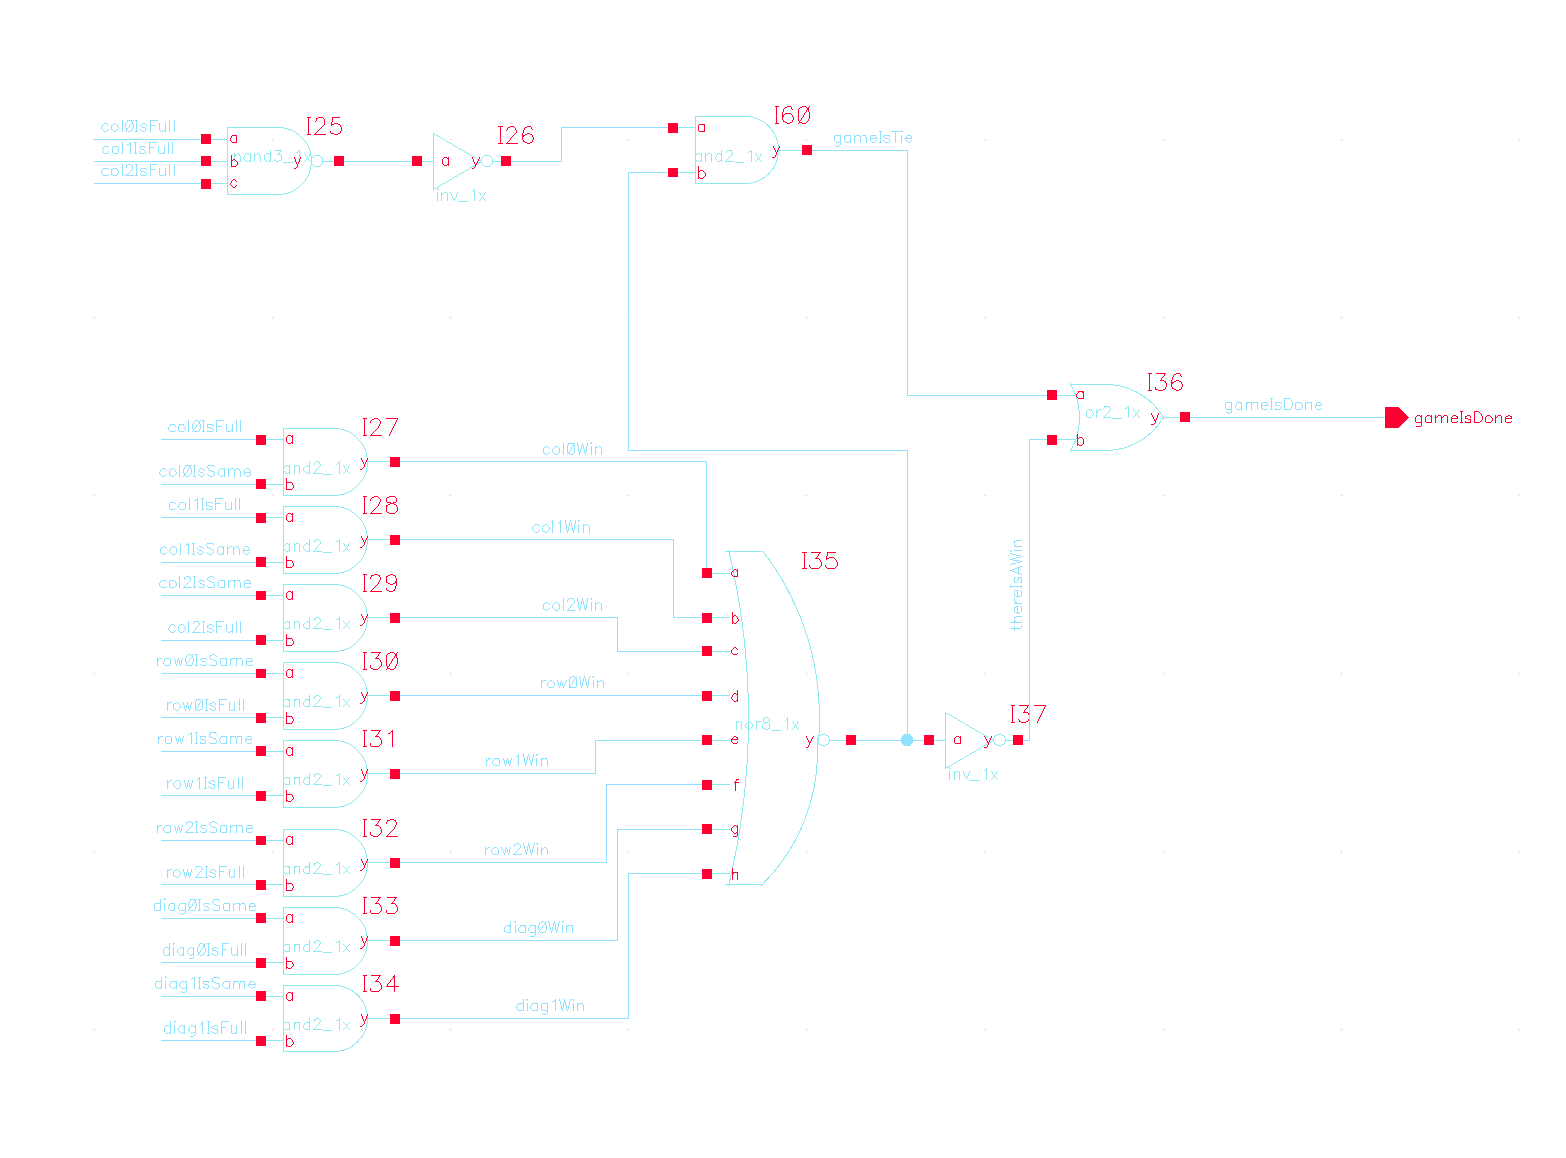
\includegraphics[width=.2\textwidth]{winLogic-schem_1}
\caption{winLogic row, column diagonal check}
\label{fig:winLogic-schem1}
\end{figure}

\begin{figure}
\centering
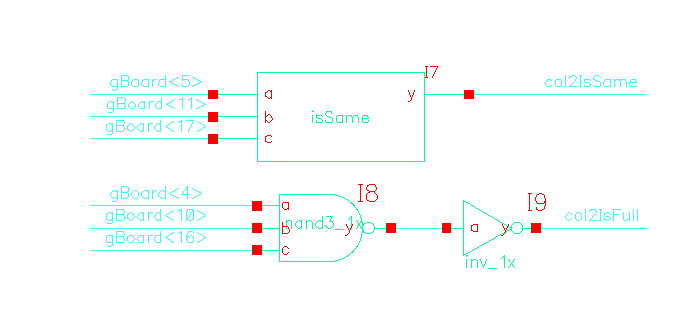
\includegraphics[width=.5\textwidth]{winLogic-schem_2}
\caption{winLogic isSame and isFull check from game-board}
\label{fig:winLogic-schem2}
\end{figure}

\begin{figure}
\centering
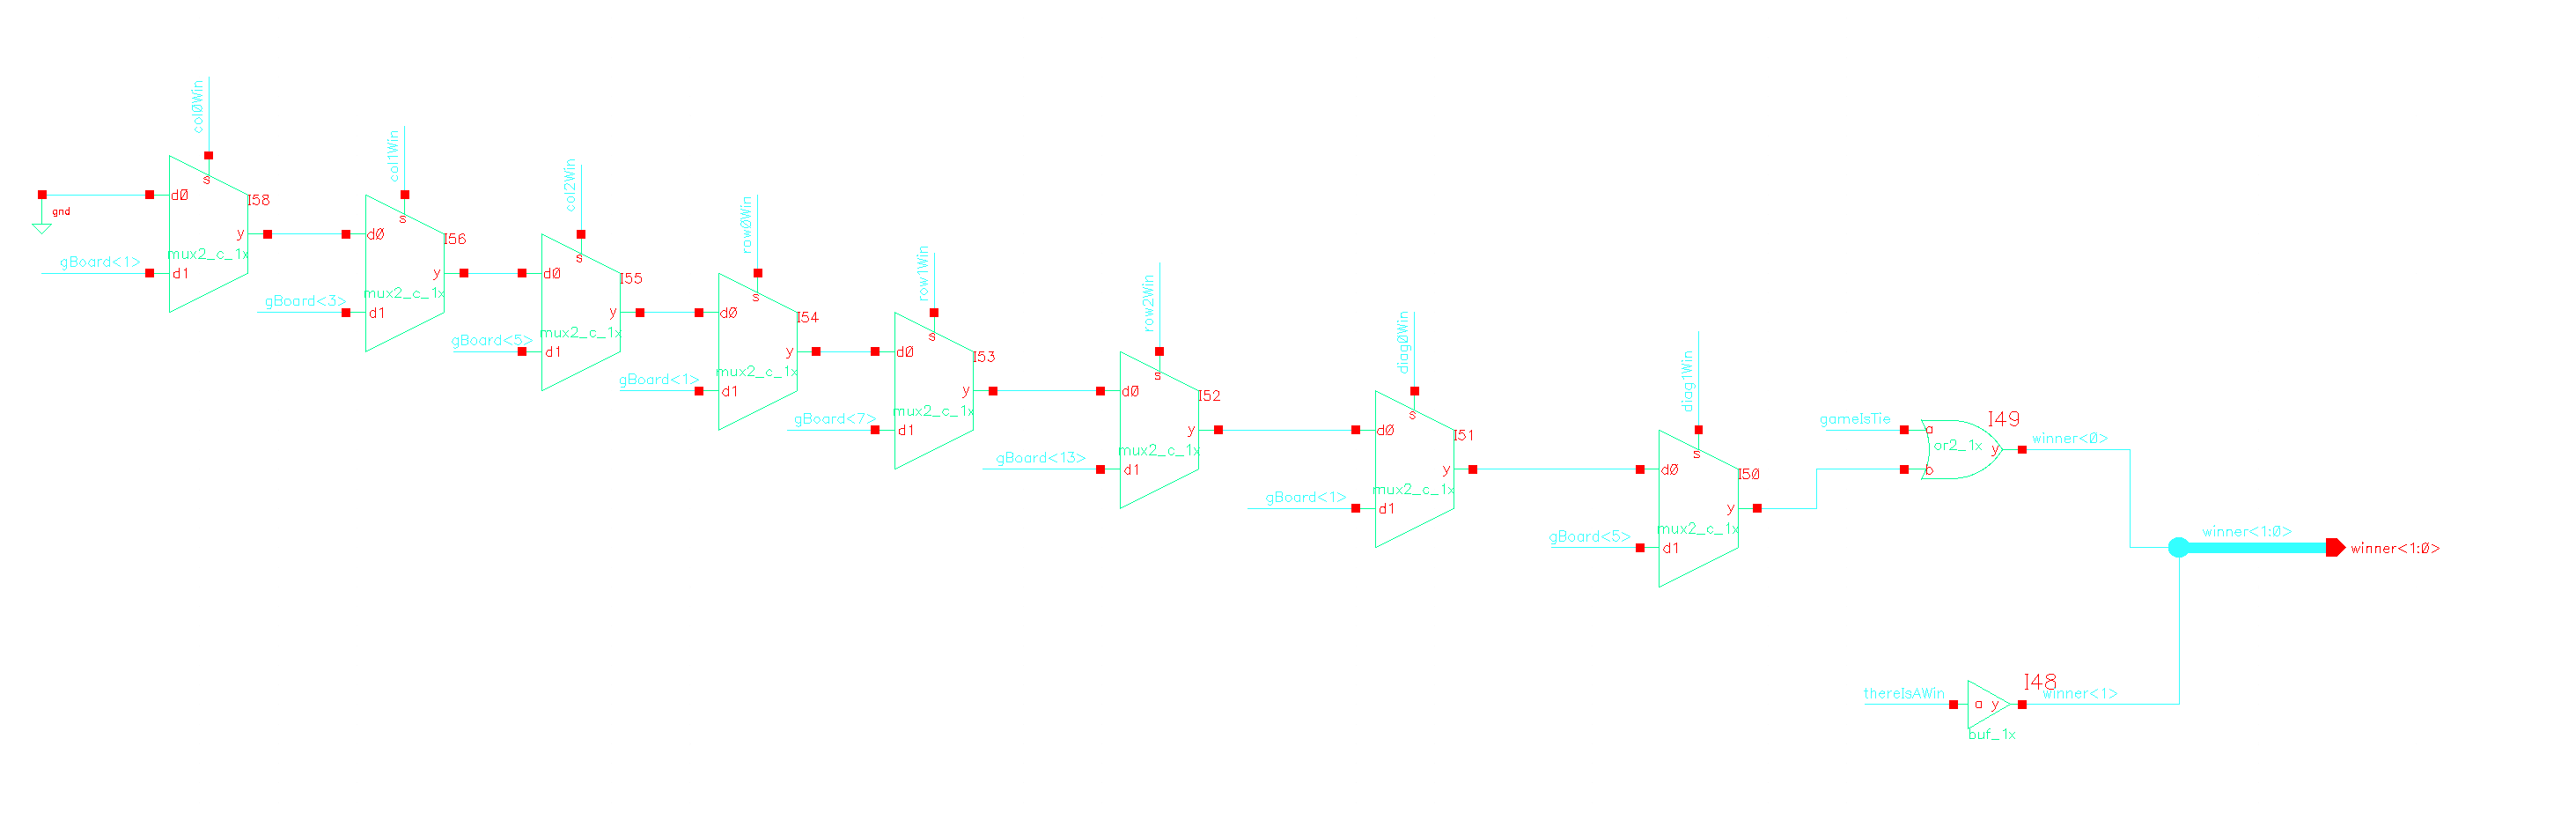
\includegraphics[width=.8\textwidth]{winLogic-schem_3}
\caption{winLogic winner select block}
\label{fig:winLogic-schem3}
\end{figure}


\subsection{\texttt{isSame} leaf cell}
\label{sec:isSame}
CMOS logic is used to check if 3 bits are identical. This cell is used to determine if the cells are taken by the same agent. The CMOS schematic can be seen in fig.~\ref{fig:isSame-cmos}.

\begin{figure}
\centering
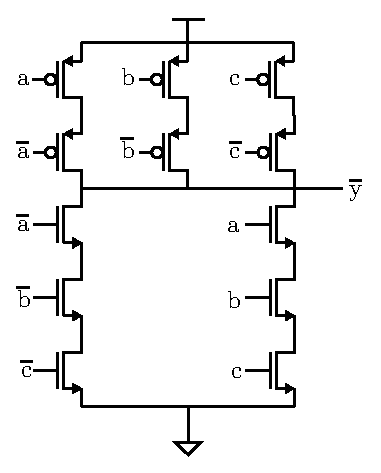
\includegraphics[width=.2\textwidth]{isSame-cmos}
\caption{isSame leaf cell logic}
\label{fig:isSame-cmos}
\end{figure}

\subsection{FSM desgin: Game Controller}
The \emph{Game Controller} contains a finite state machine (FSM) to decide when each player has to play and whether or not the game is done. A state transition diagram for the game controller FSM is shown in figure~\ref{fig:gameController-FSM}.

\begin{figure}
\centering
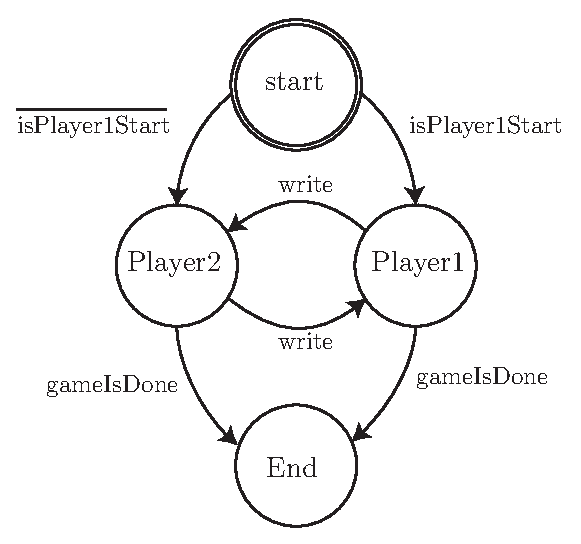
\includegraphics[width=.3\textwidth]{gameController-FSM}
\caption{Game Controller Finite-State-Machine}
\label{fig:gameController-FSM}
\end{figure}




\begin{thebibliography}{widest entry}
\bibitem{e85-book}
  David Harris \& Sarah Harris,
  \emph{Digital Design and Computer Architecture},
  Morgan Kaufmann; 2nd edition,
  2012.
\bibitem{flip-flop-paper}
 Crowley, Kevin \& Siegler, Robert S.
  \emph{Flexible Strategy Use in Young Children's Tic-Tac-Toe},
  Cognitive Science; Issue 4, Volume 2,
  1993.
 \bibitem{checkersReport}
 Max Korbel \& Ian Jimenez
  \emph{Simplified Checkers},
  E158: Introduction to CMOS VLSI Design Lab Report,
  2011. 

\end{thebibliography}


%\appendices
\appendix
\section{Schematics \& layouts}

% gameController
\subsection{gameController}
\begin{figure}[H]
\centering
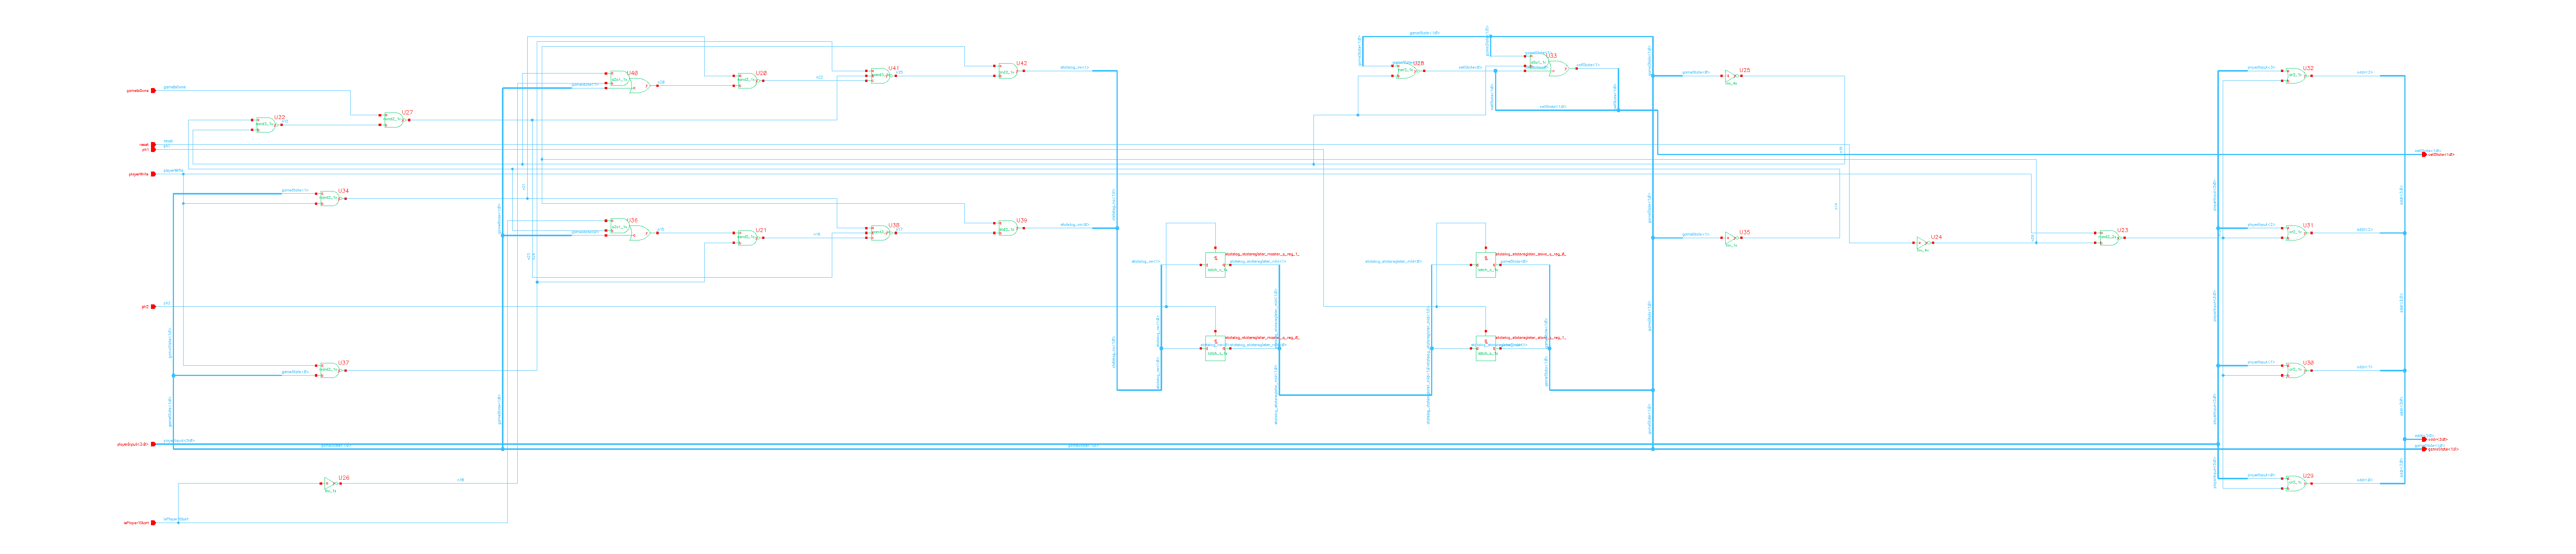
\includegraphics[width=.9\textwidth]{gameController-schematic}
\caption{gameController synthetized schematic}
\label{fig:gameController-schematic}
\end{figure}

\begin{figure}[H]
\centering
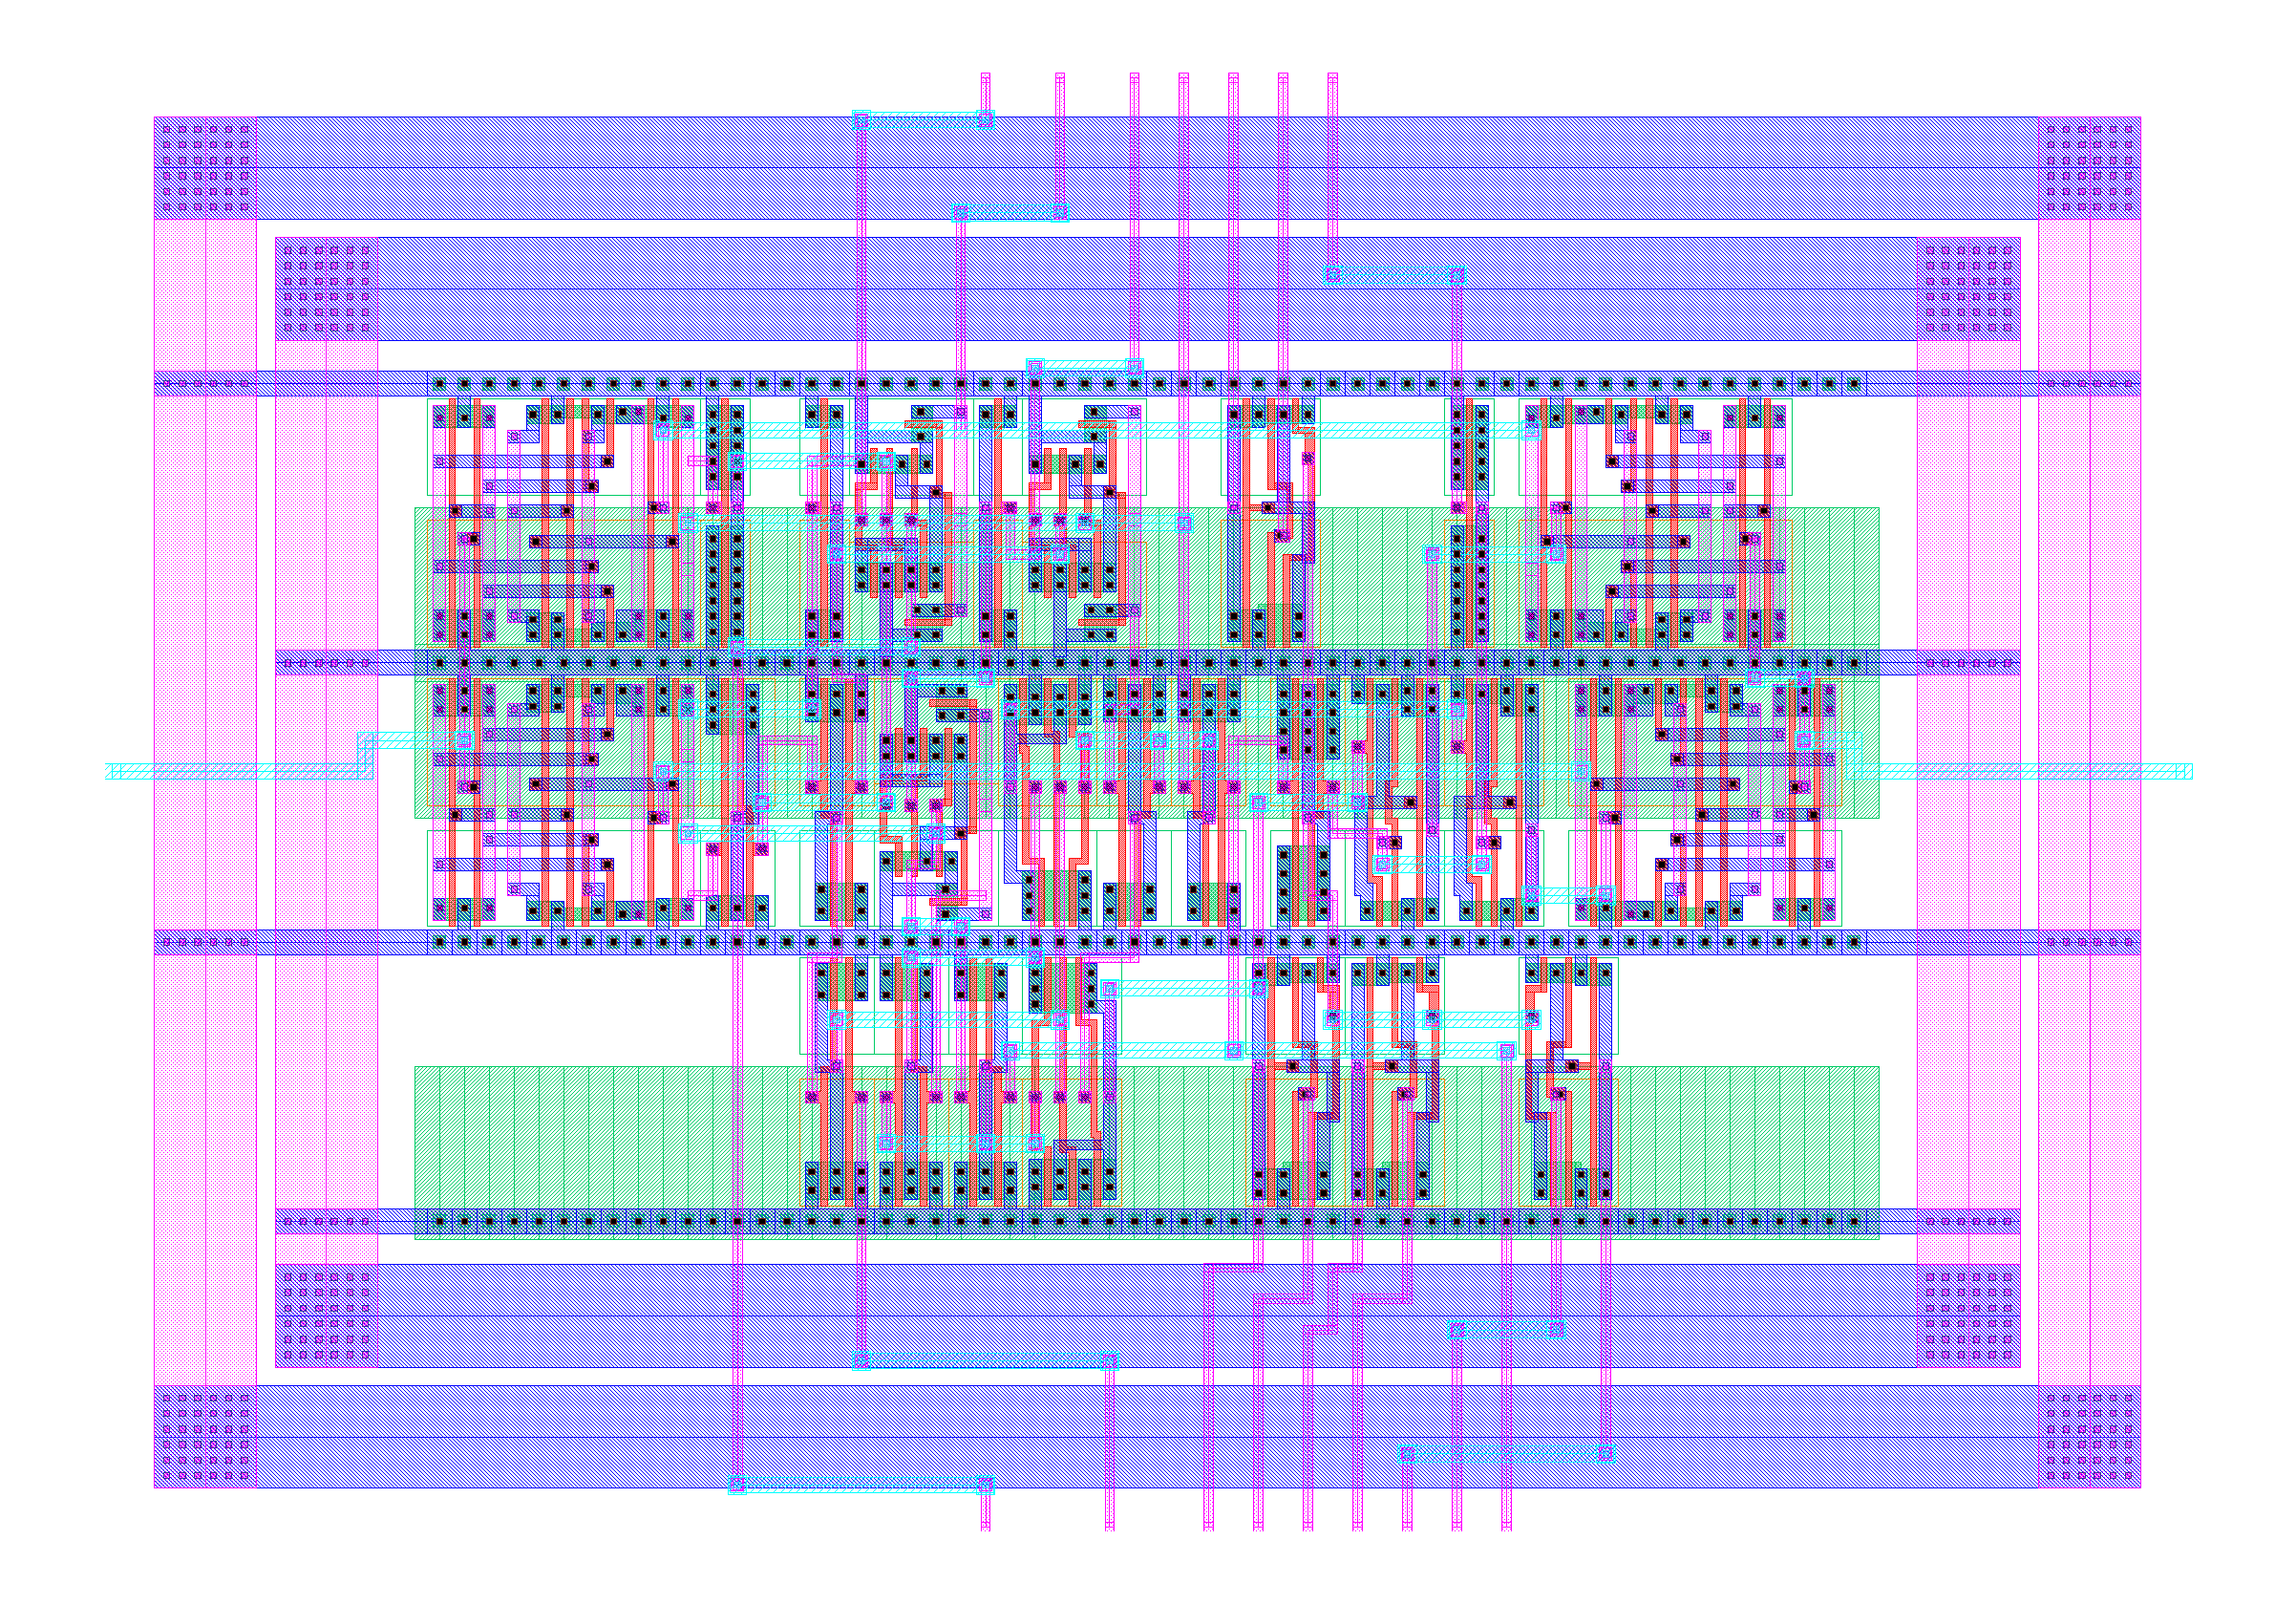
\includegraphics[width=.9\textwidth]{gameController-layout}
\caption{gameController synthetized layout}
\label{fig:gameController-layout}
\end{figure}

% winLogic
\subsection{winLogic}
\begin{figure}[H]
\centering
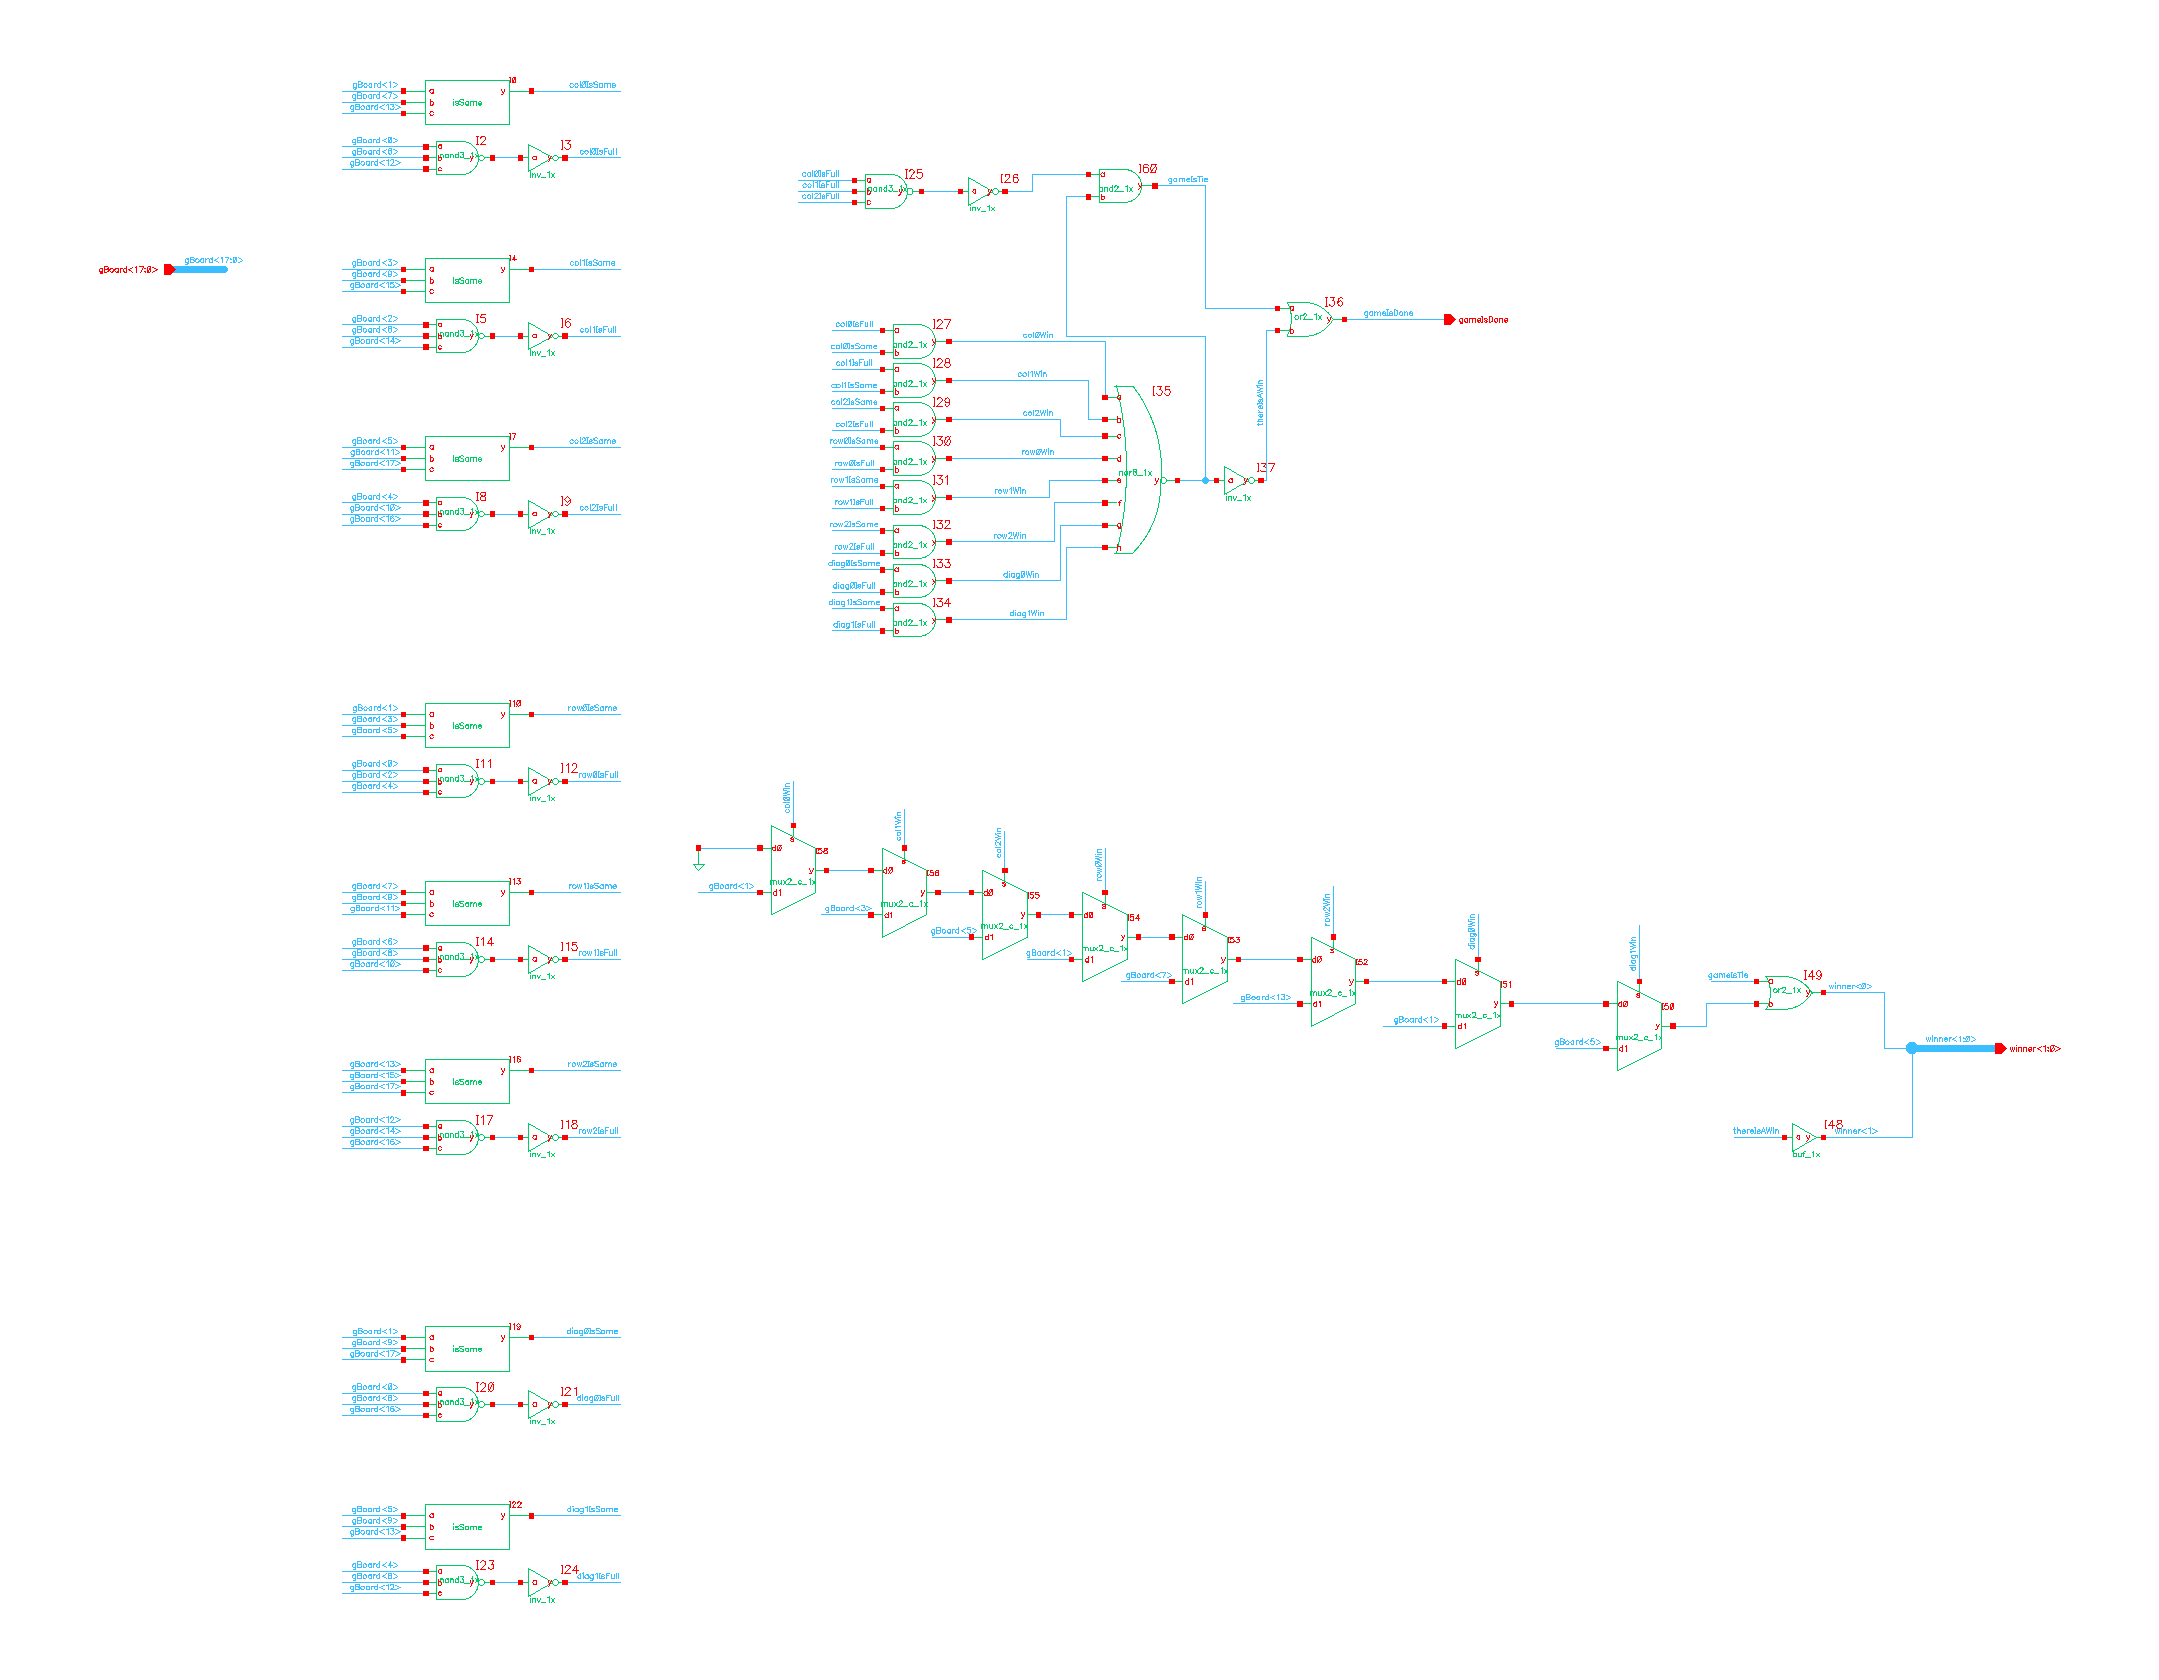
\includegraphics[width=.9\textwidth]{winLogic-schematic}
\caption{winLogic schematic}
\label{fig:winLogic-schematic}
\end{figure}

\begin{figure}[H]
\centering
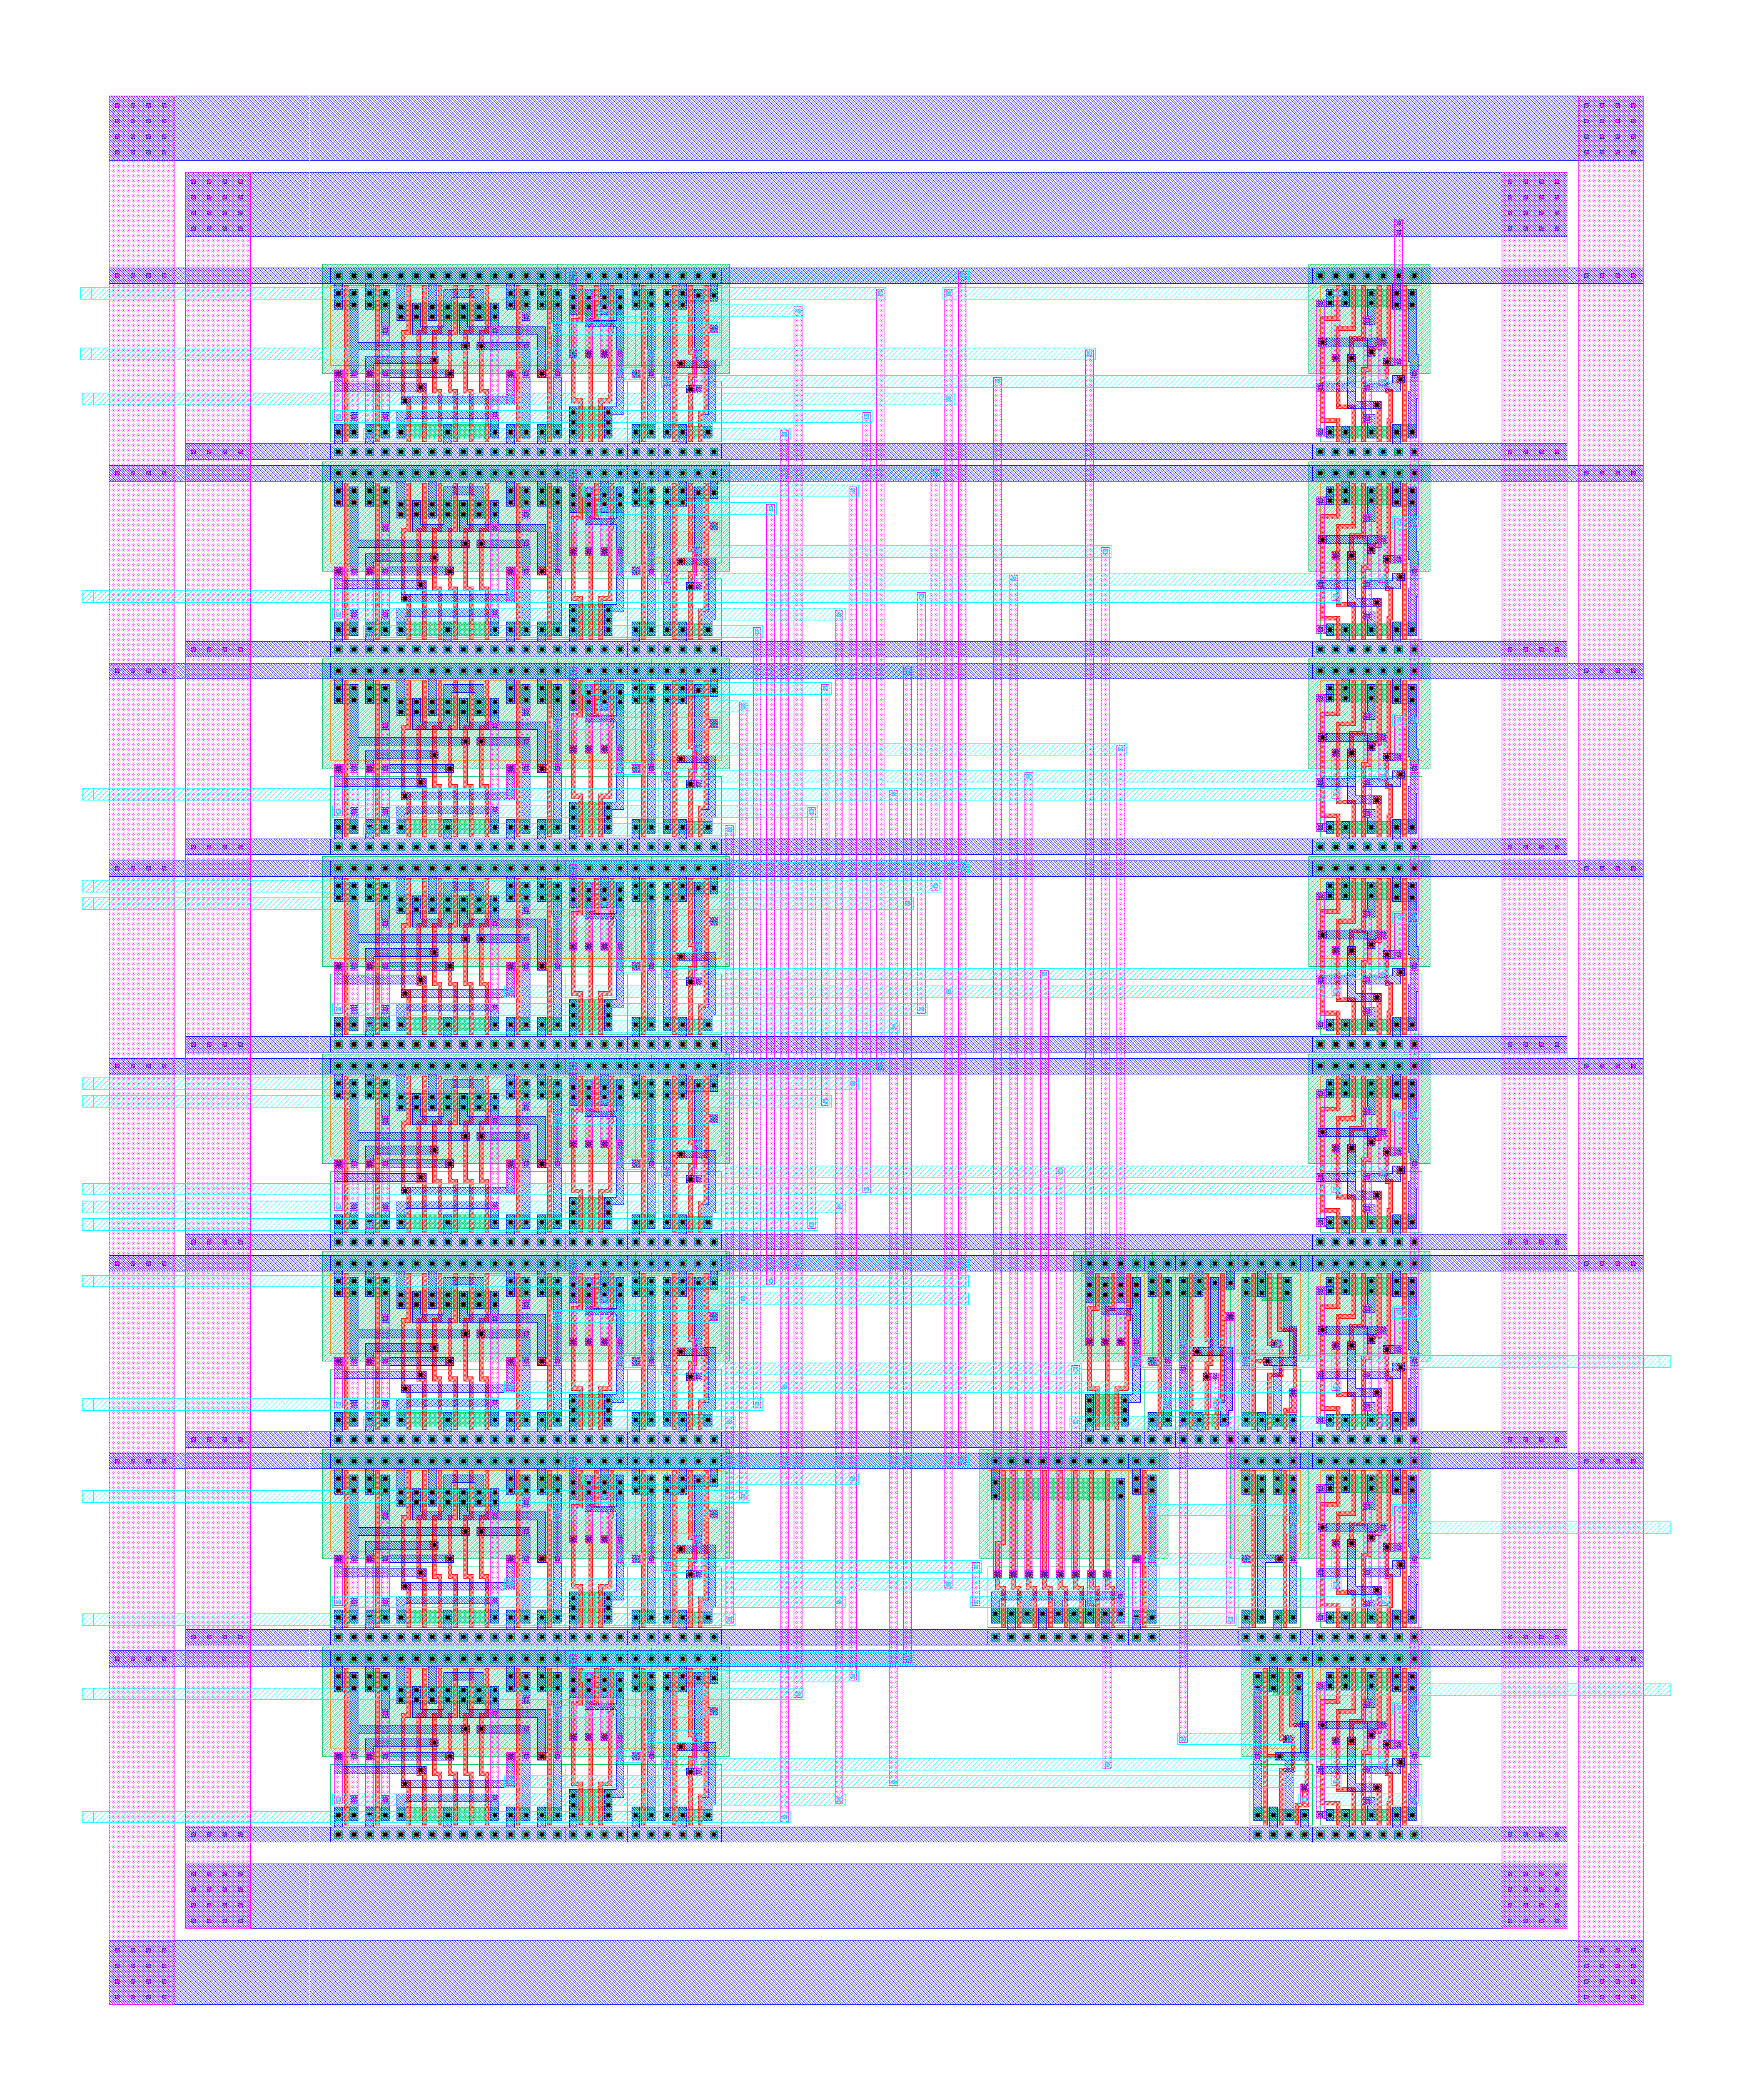
\includegraphics[width=.9\textwidth]{winLogic-layout}
\caption{winLogic layout}
\label{fig:winLogic-layout}
\end{figure}

% isSame
\subsubsection{iSame leaf cell}
\begin{figure}[H]
\centering
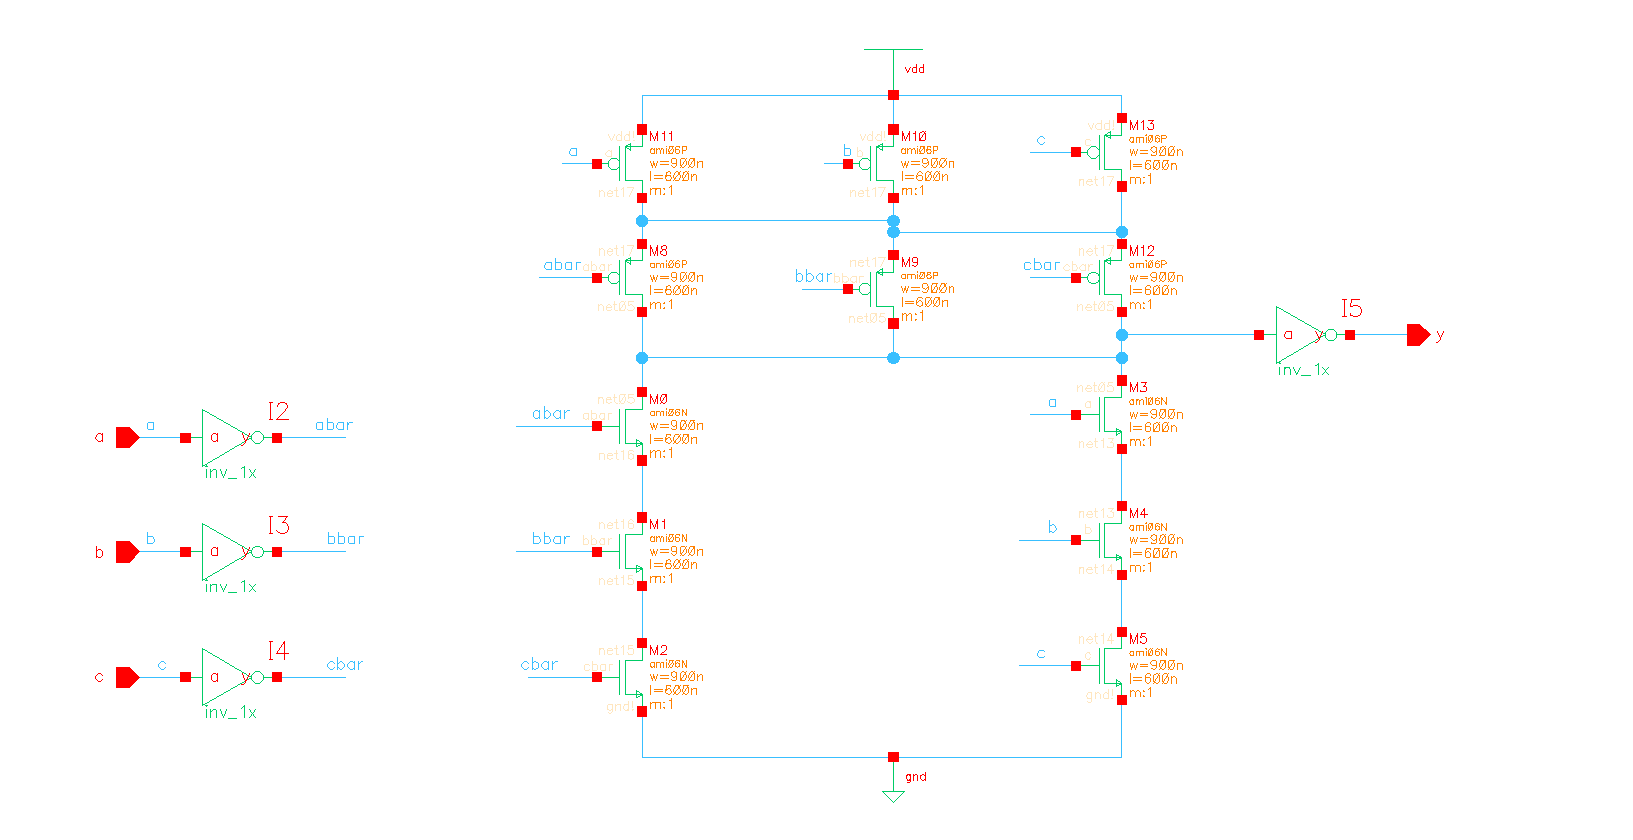
\includegraphics[width=0.9\textwidth]{isSame-schematic}
\caption{isSame leaf cell schematic}
\label{fig:isSame-schematic}
\end{figure}

\begin{figure}[H]
\centering
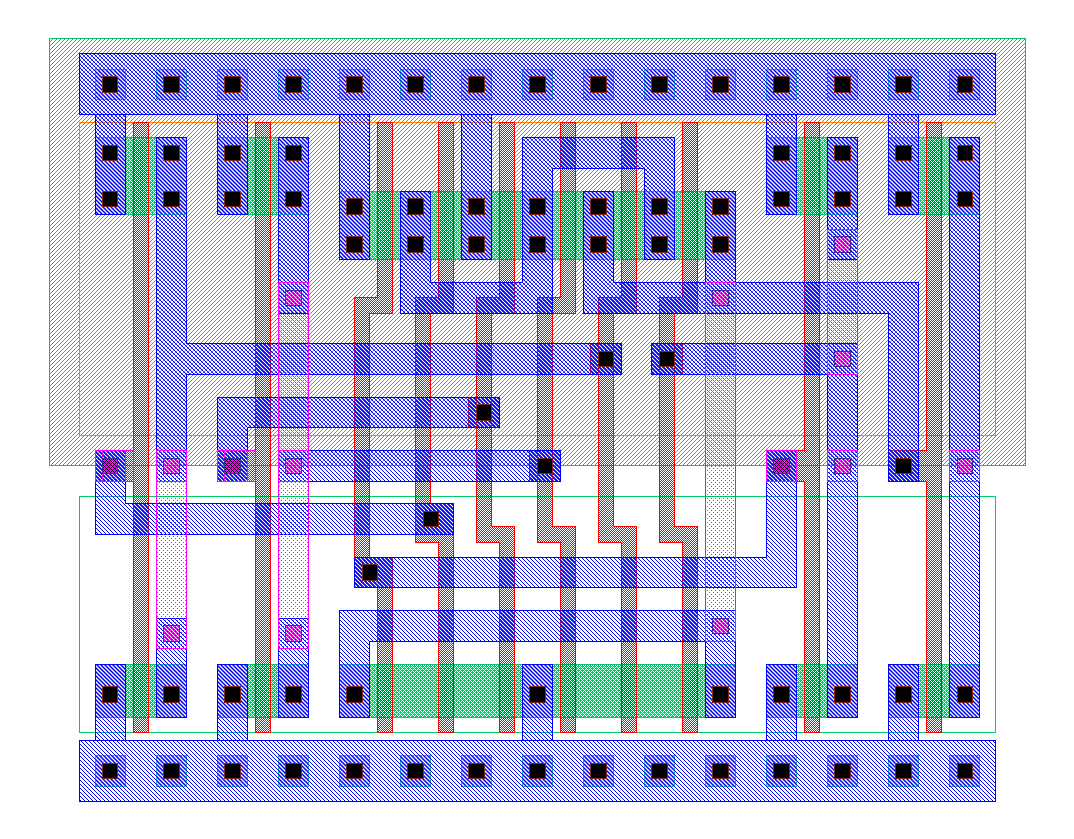
\includegraphics[width=0.9\textwidth]{isSame-layout}
\caption{isSame leaf cell layout}
\label{fig:isSame-layout}
\end{figure}

% nor8_1x
\subsubsection{nor8\_1x leaf cell}
\begin{figure}[H]
\centering
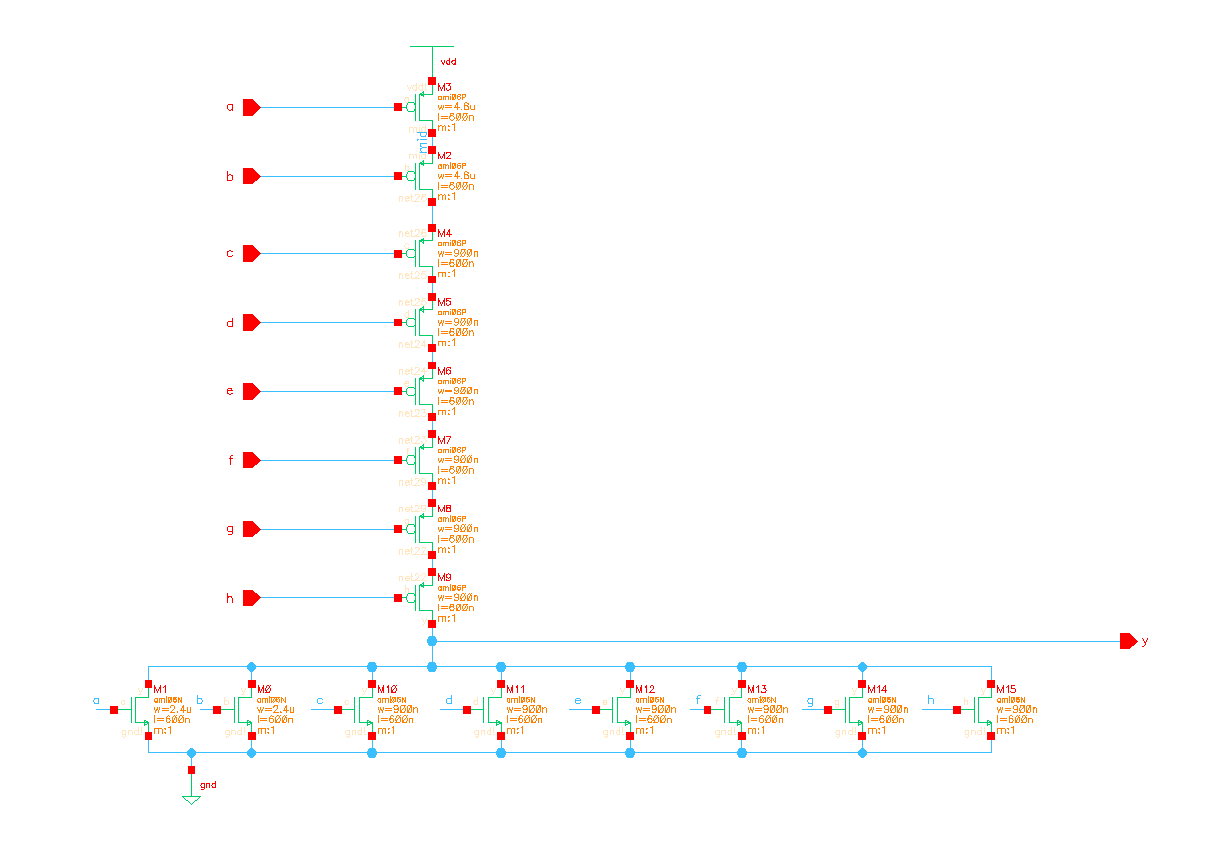
\includegraphics[width=.9\textwidth]{nor8_1x-cmos_sch}
\caption{nor8\_1x cmos schematic}
\label{fig:nor8-schematic}
\end{figure}

\begin{figure}[H]
\centering
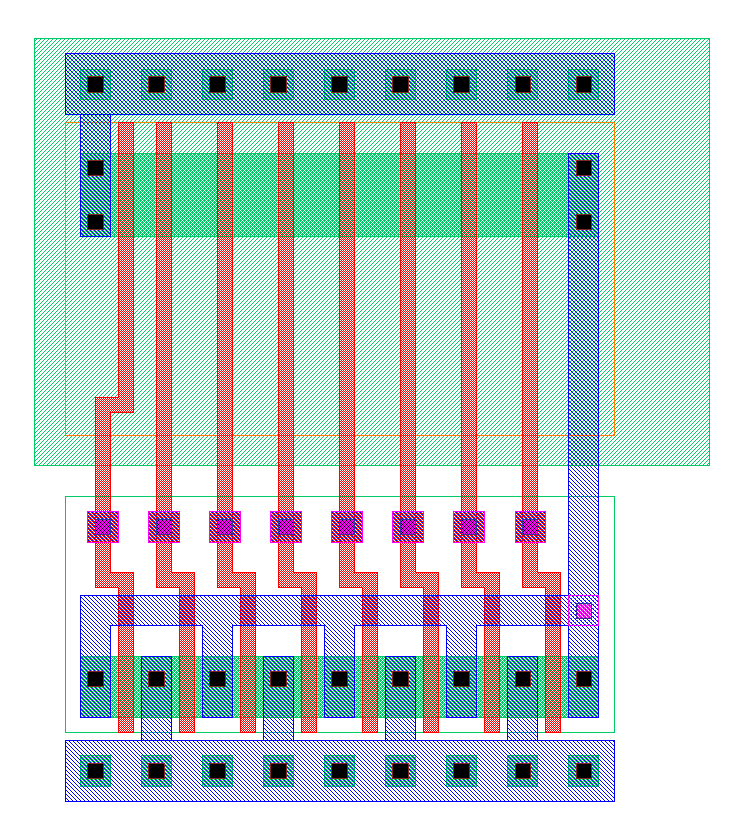
\includegraphics[width=.9\textwidth]{nor8_1x-layout}
\caption{nor8\_1x layout}
\label{fig:nor8-layout}
\end{figure}

% memArray
\subsection{memArray}
\begin{figure}[H]
\centering
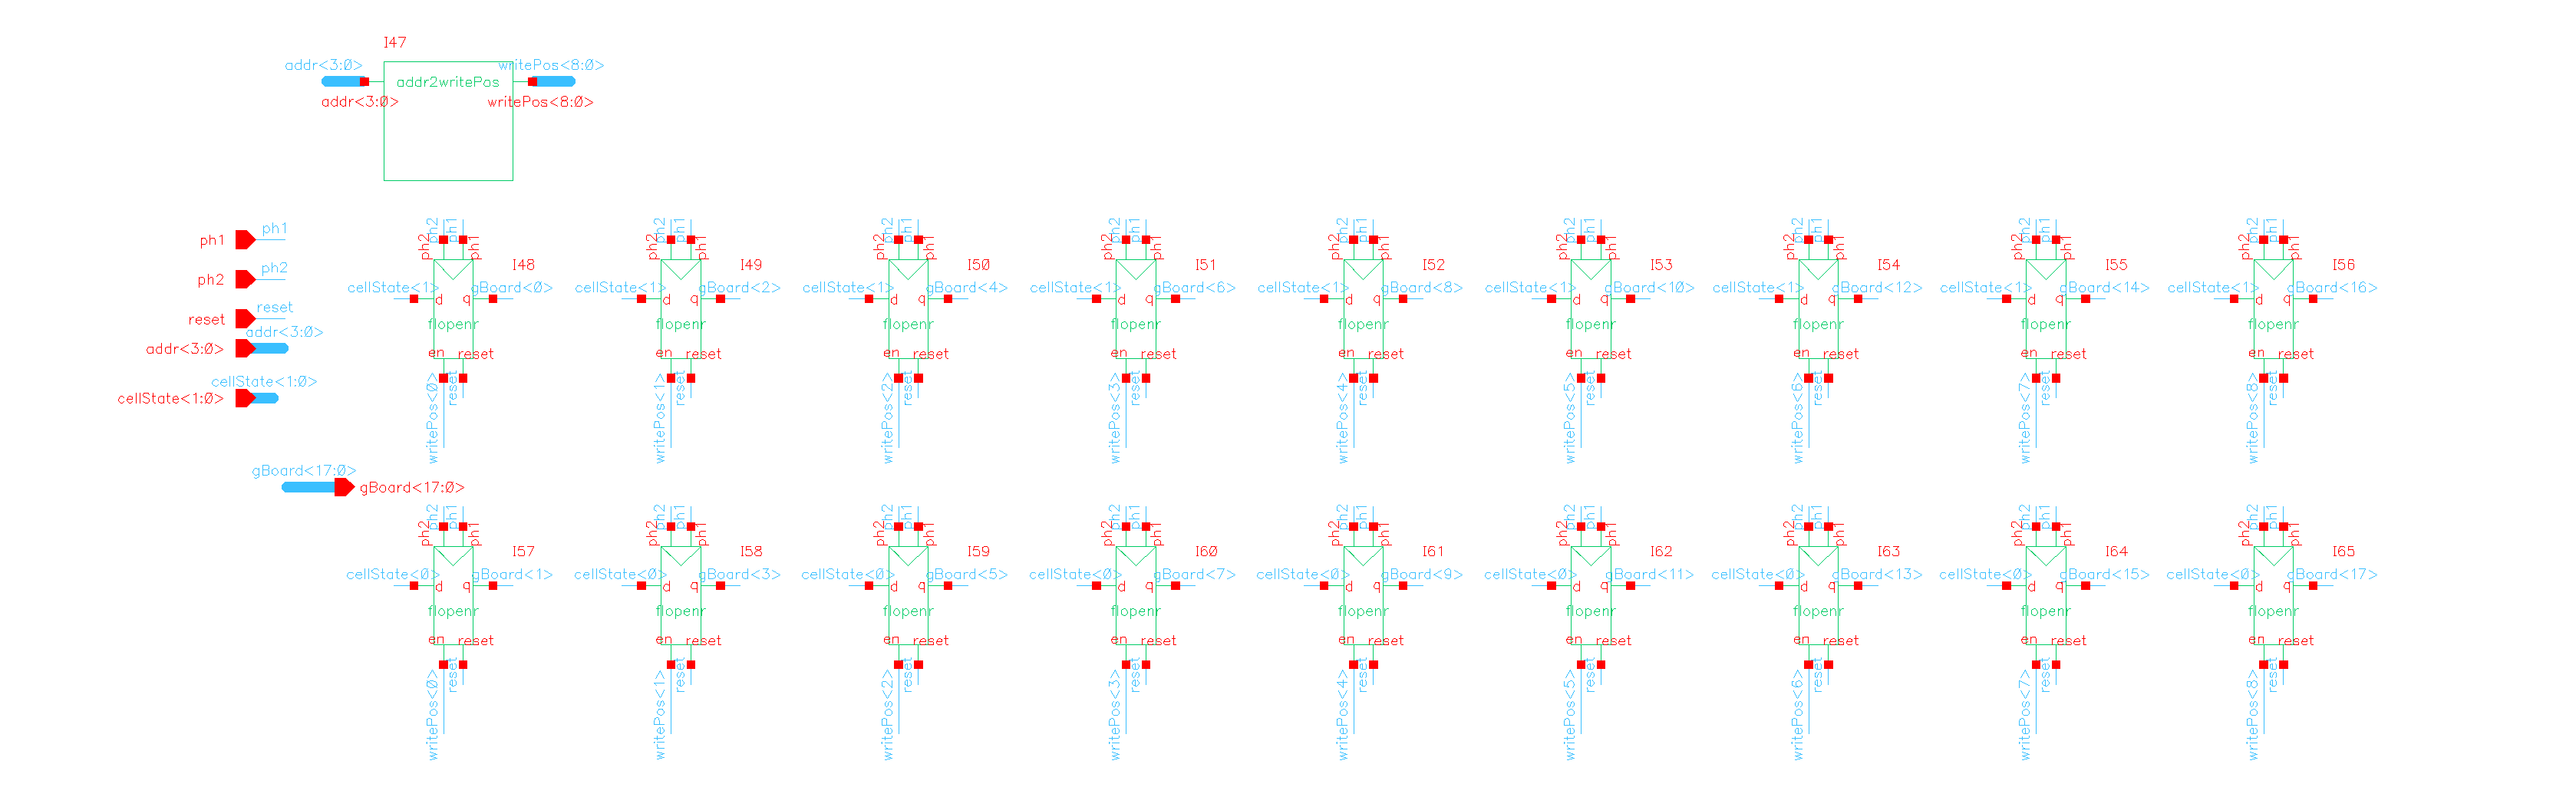
\includegraphics[width=.9\textwidth]{memArray-schematic}
\caption{memArray schematic}
\label{fig:memArray-schematic}
\end{figure}

\begin{figure}[H]
\centering
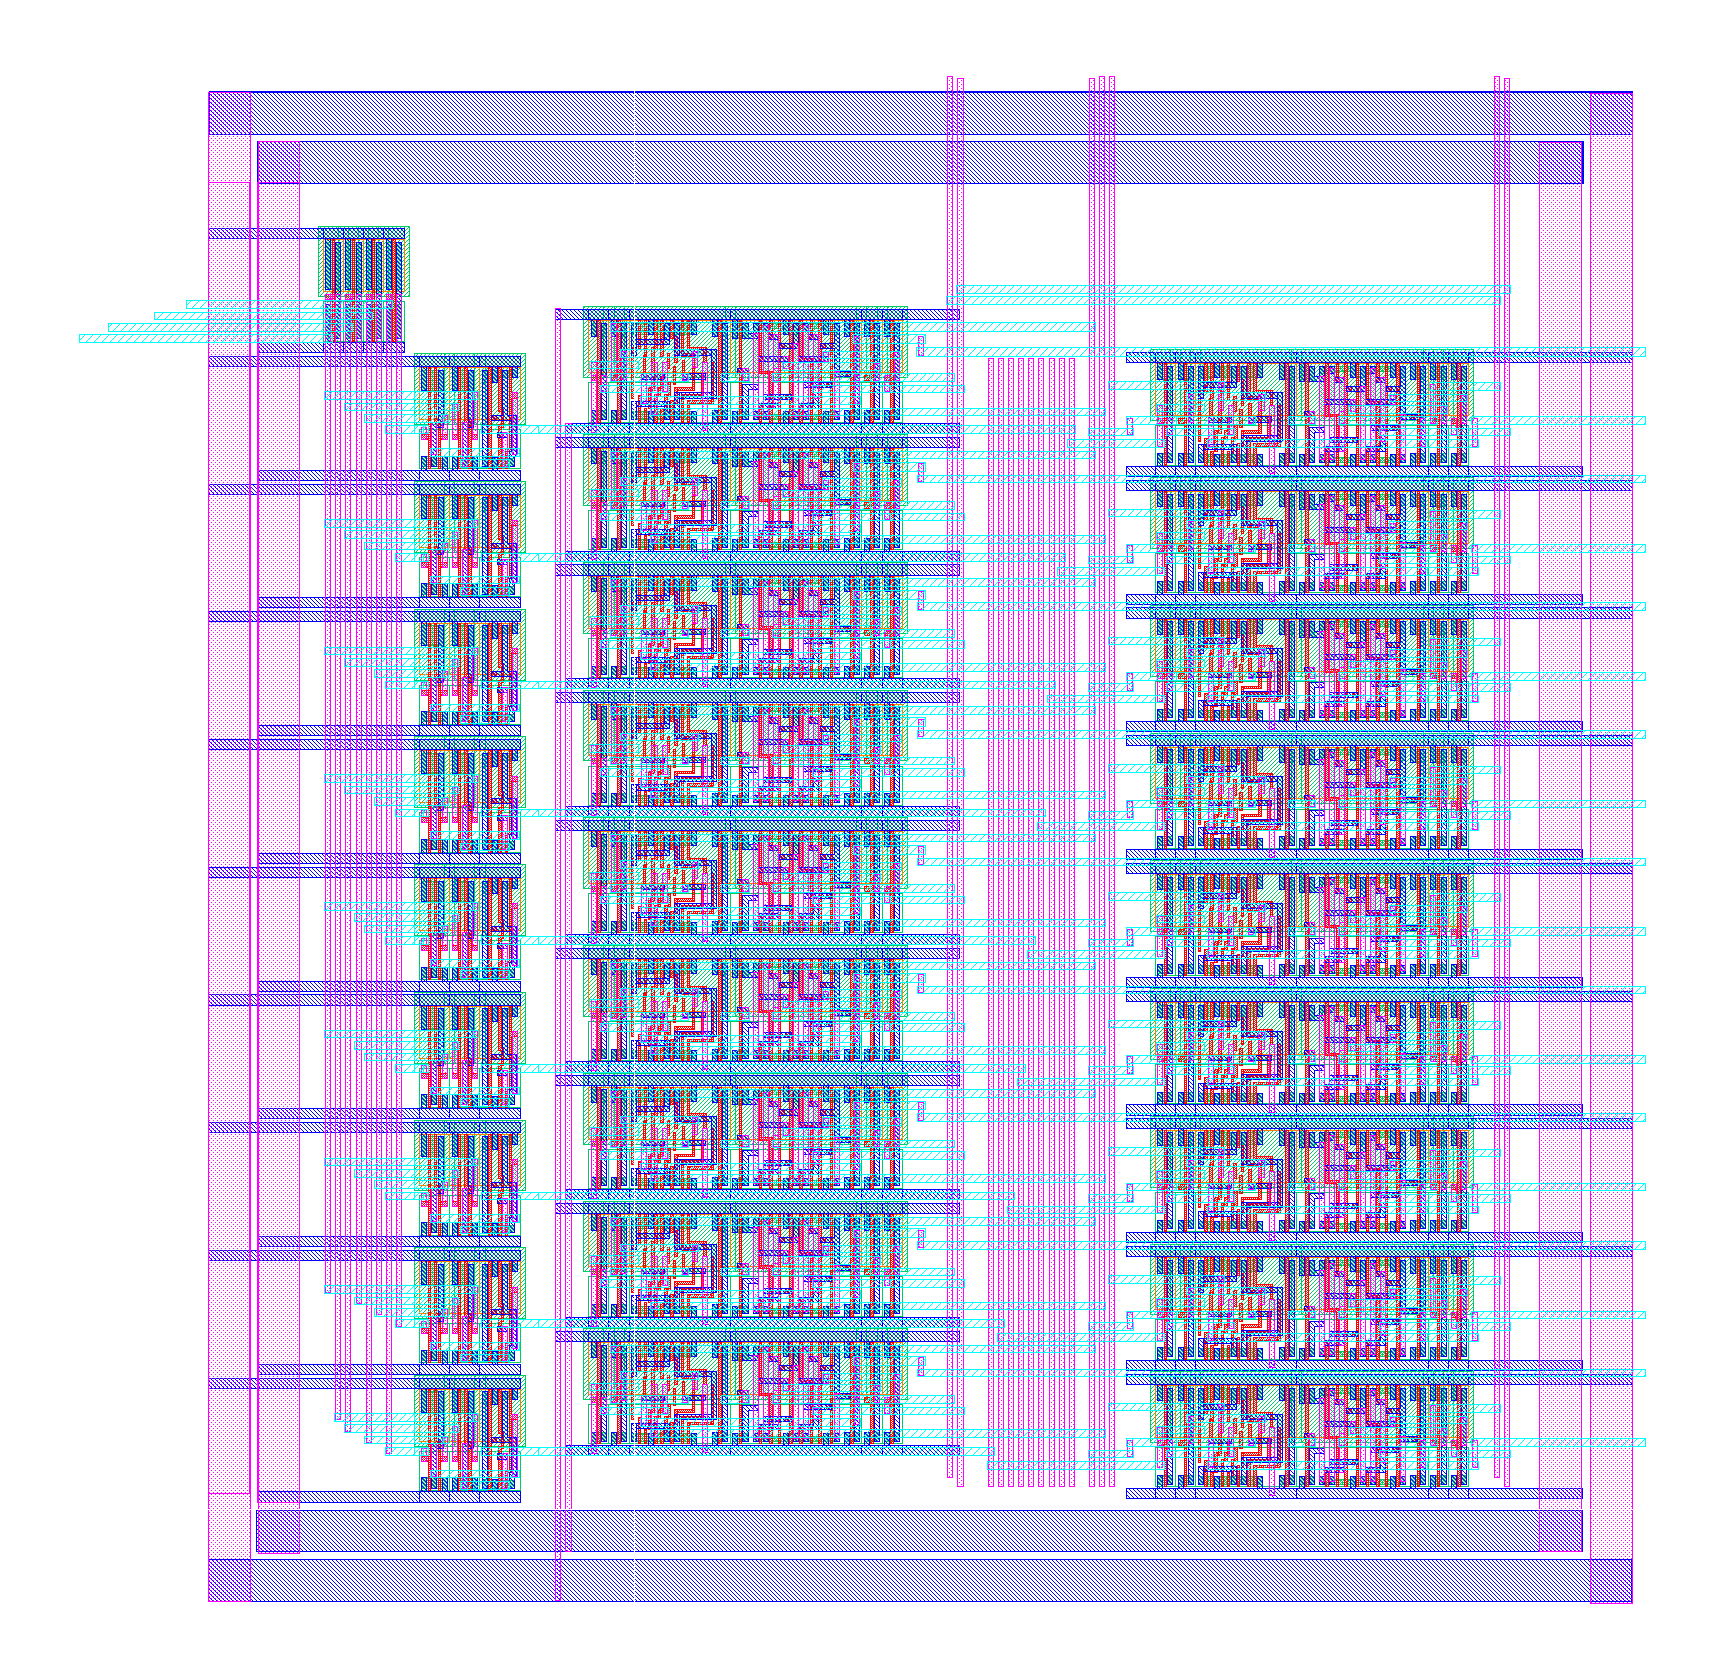
\includegraphics[width=.9\textwidth]{memArray-layout}
\caption{memArray layout}
\label{fig:memArray-layout}
\end{figure}

\subsubsection{addr2pos}
\begin{figure}[H]
\centering
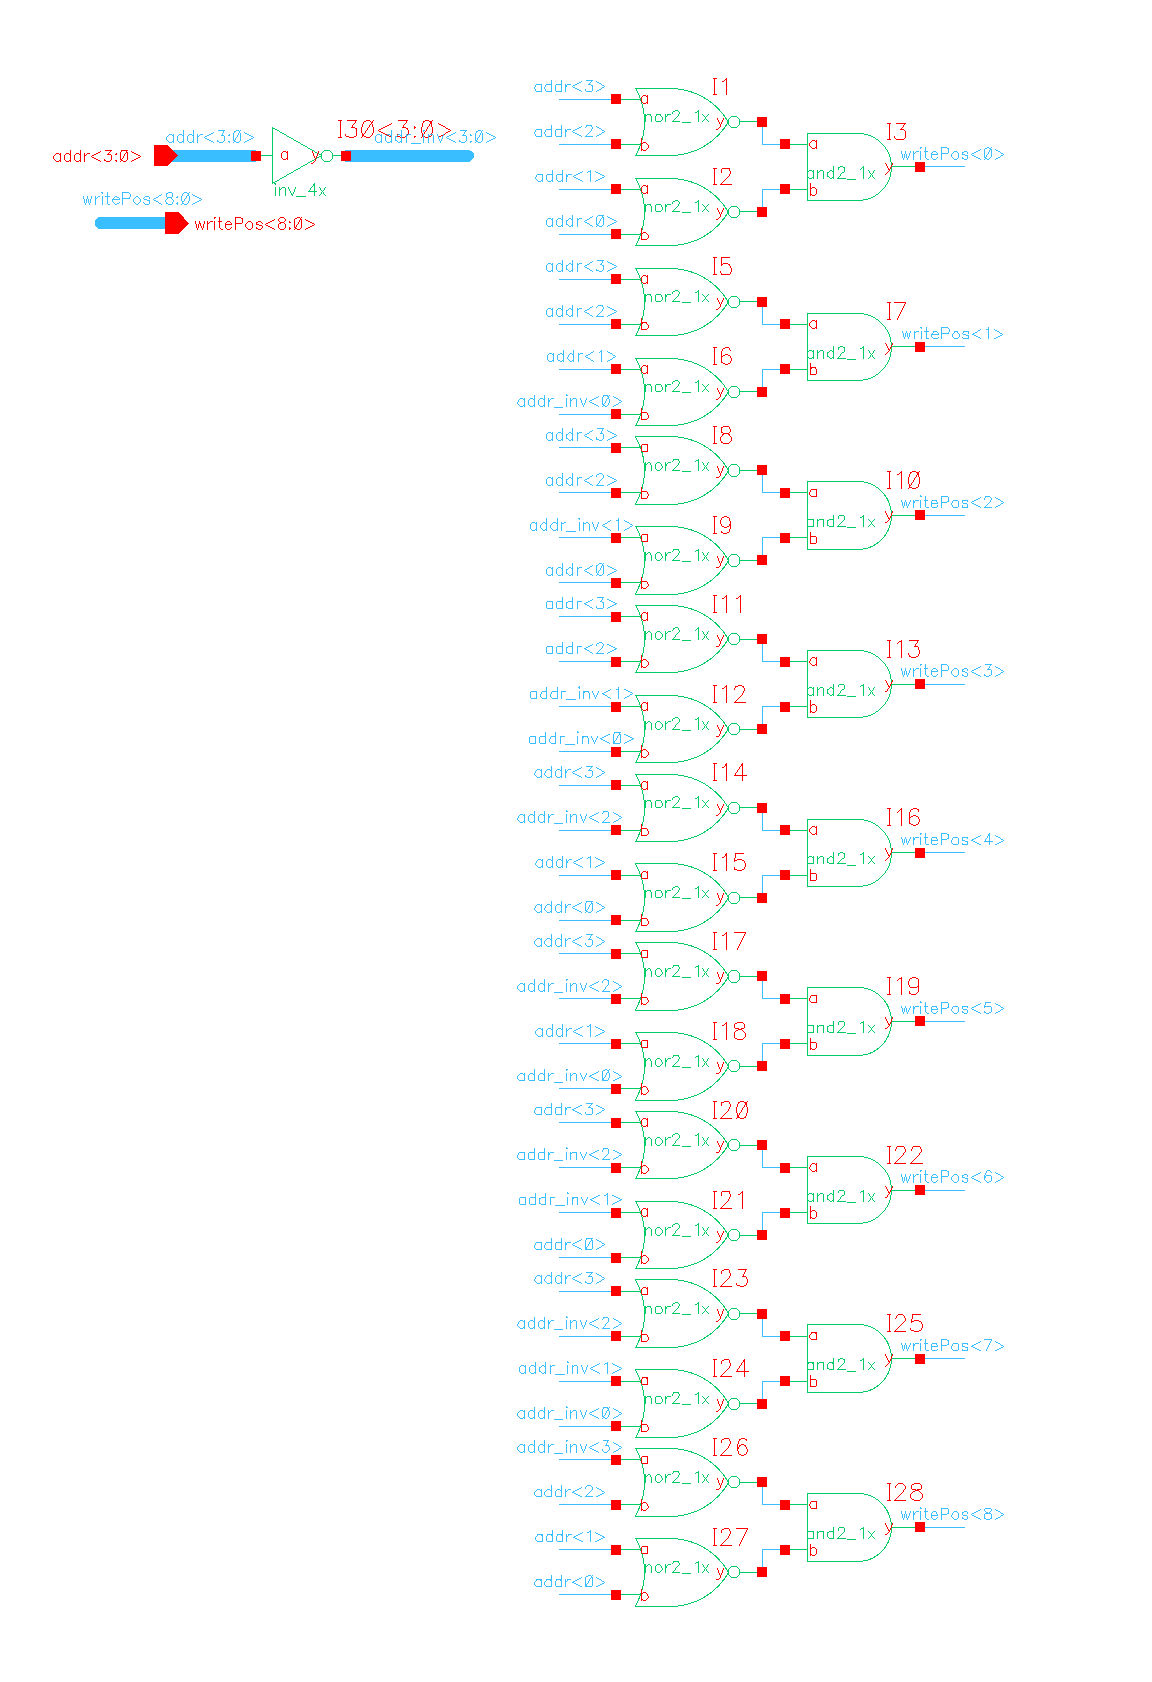
\includegraphics[width=.9\textwidth]{addr2writePos-schematic}
\caption{addr2writePos layout}
\label{fig:addr2writePos-schematic}
\end{figure}

\begin{figure}[H]
\centering
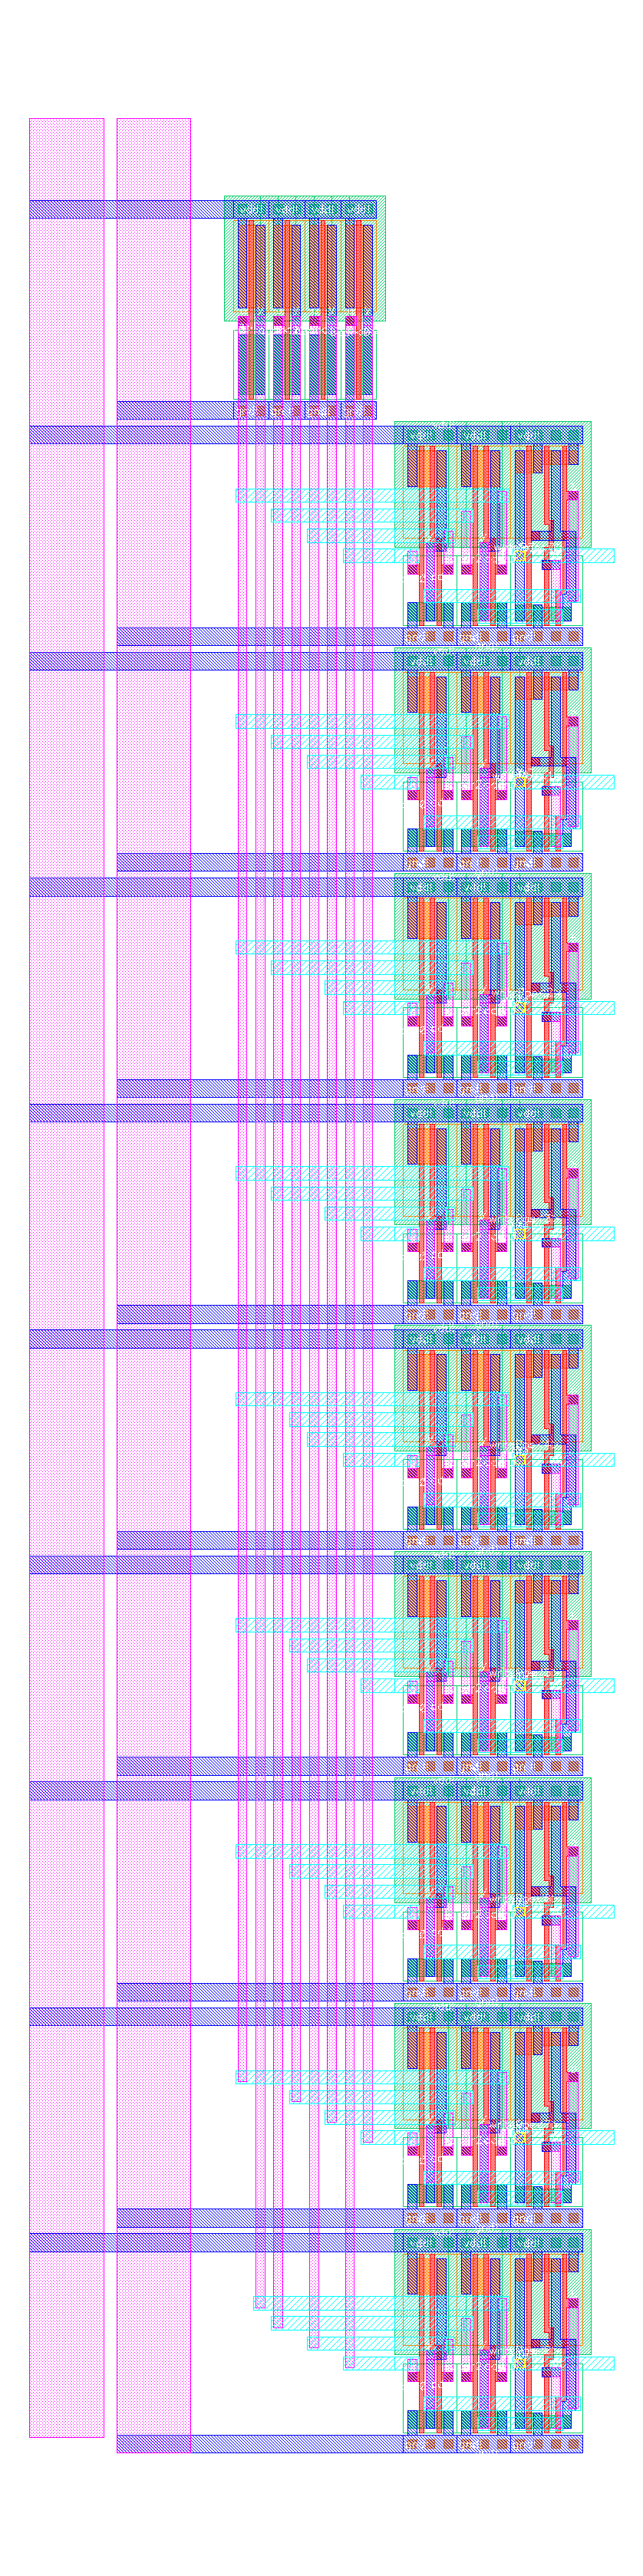
\includegraphics[height=.8\paperheight]{addr2writePos-layout}
\caption{addr2writePos layout}
\label{fig:addr2writePos-layout}
\end{figure}

\subsubsection{flopenr}
\begin{figure}[H]
\centering
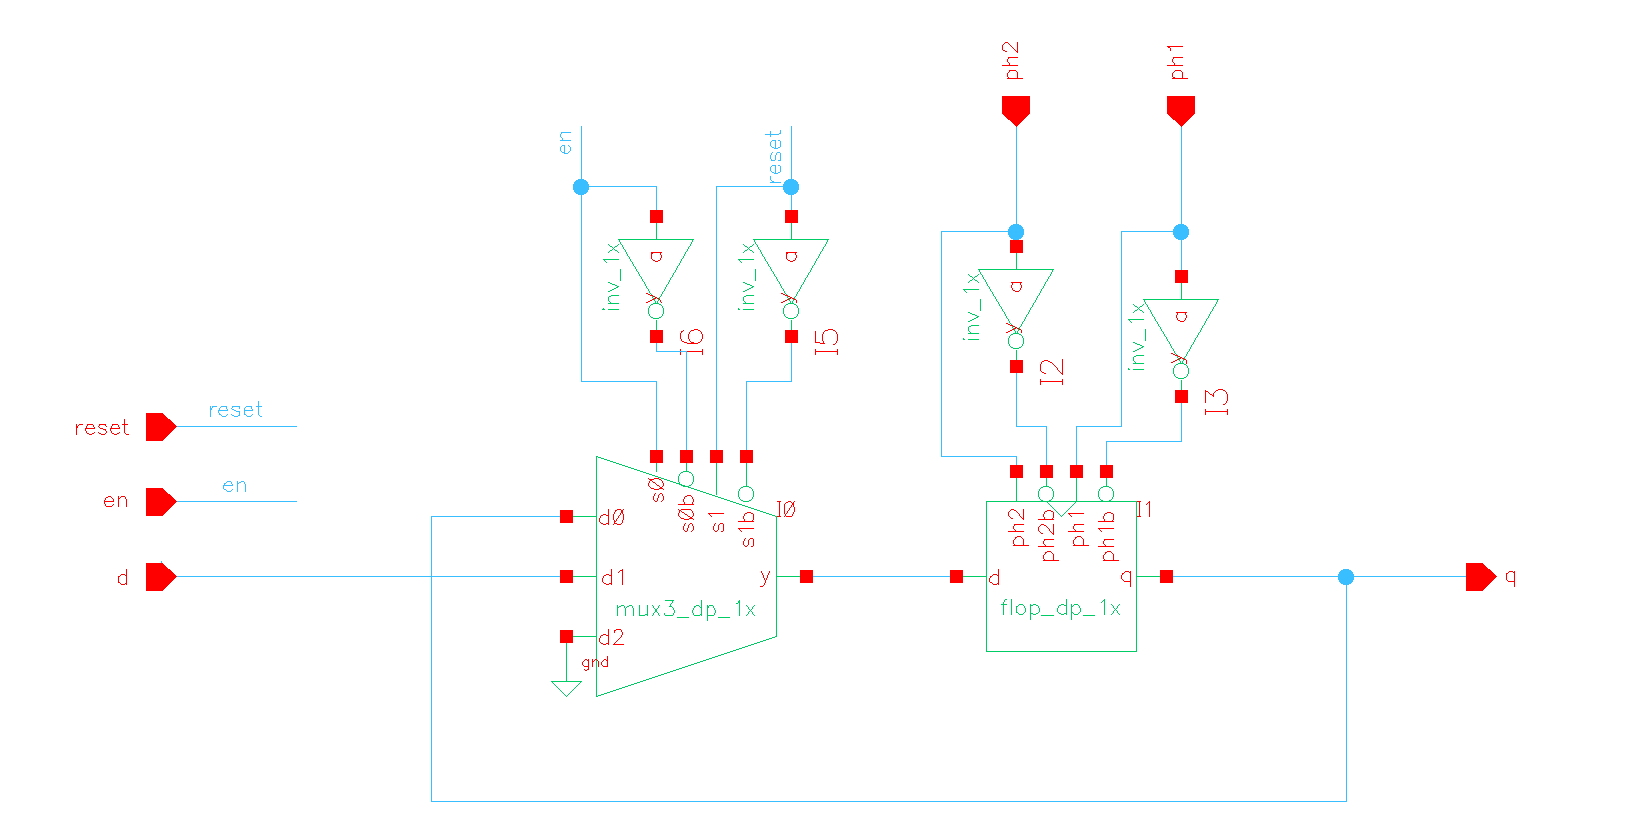
\includegraphics[width=.9\textwidth]{flopenr-schematic}
\caption{flopenr layout}
\label{fig:flopenr-schematic}
\end{figure}

\begin{figure}[H]
\centering
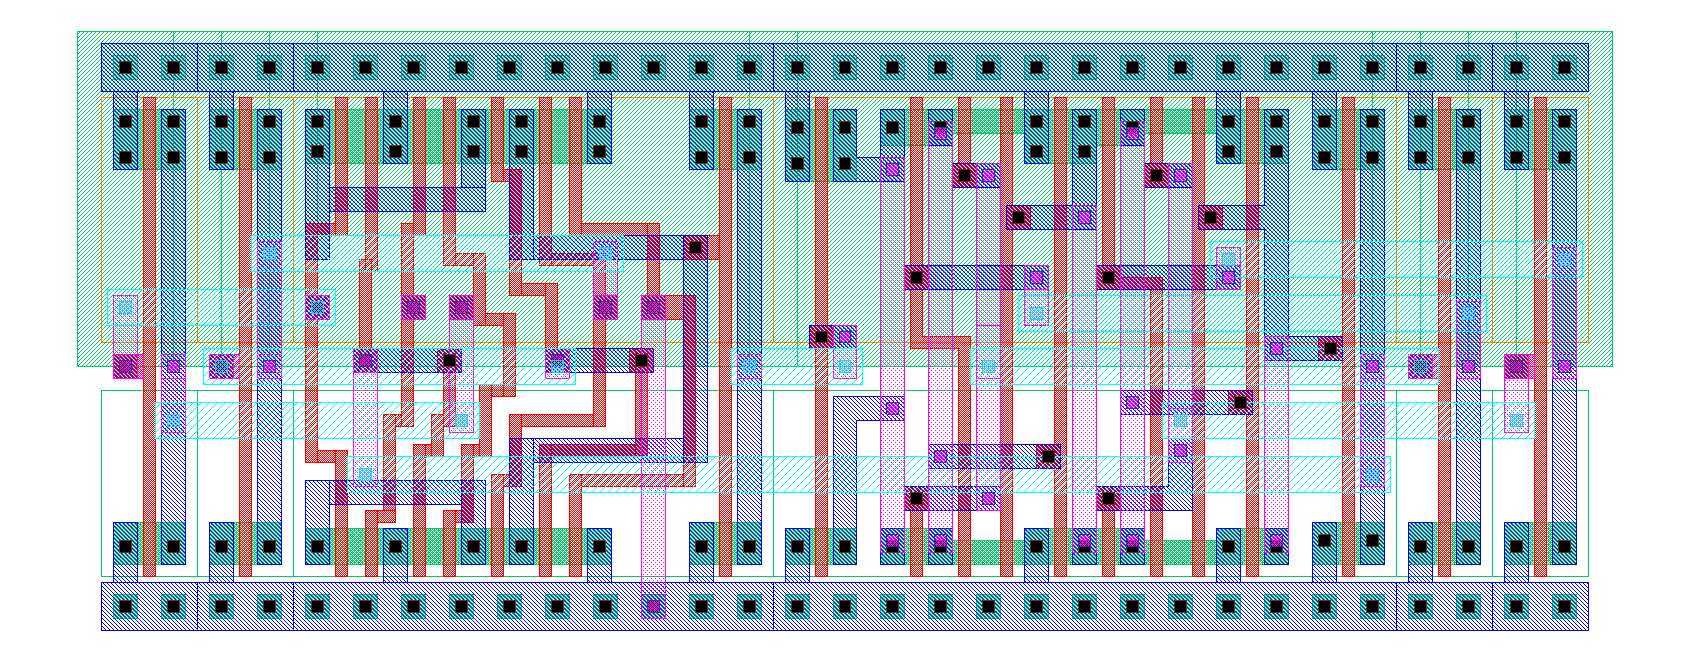
\includegraphics[width=.9\textwidth]{flopenr-layout}
\caption{flopenr layout}
\label{fig:flopenr-layout}
\end{figure}


\subsection{Padframe}
\begin{figure}[H]
\centering
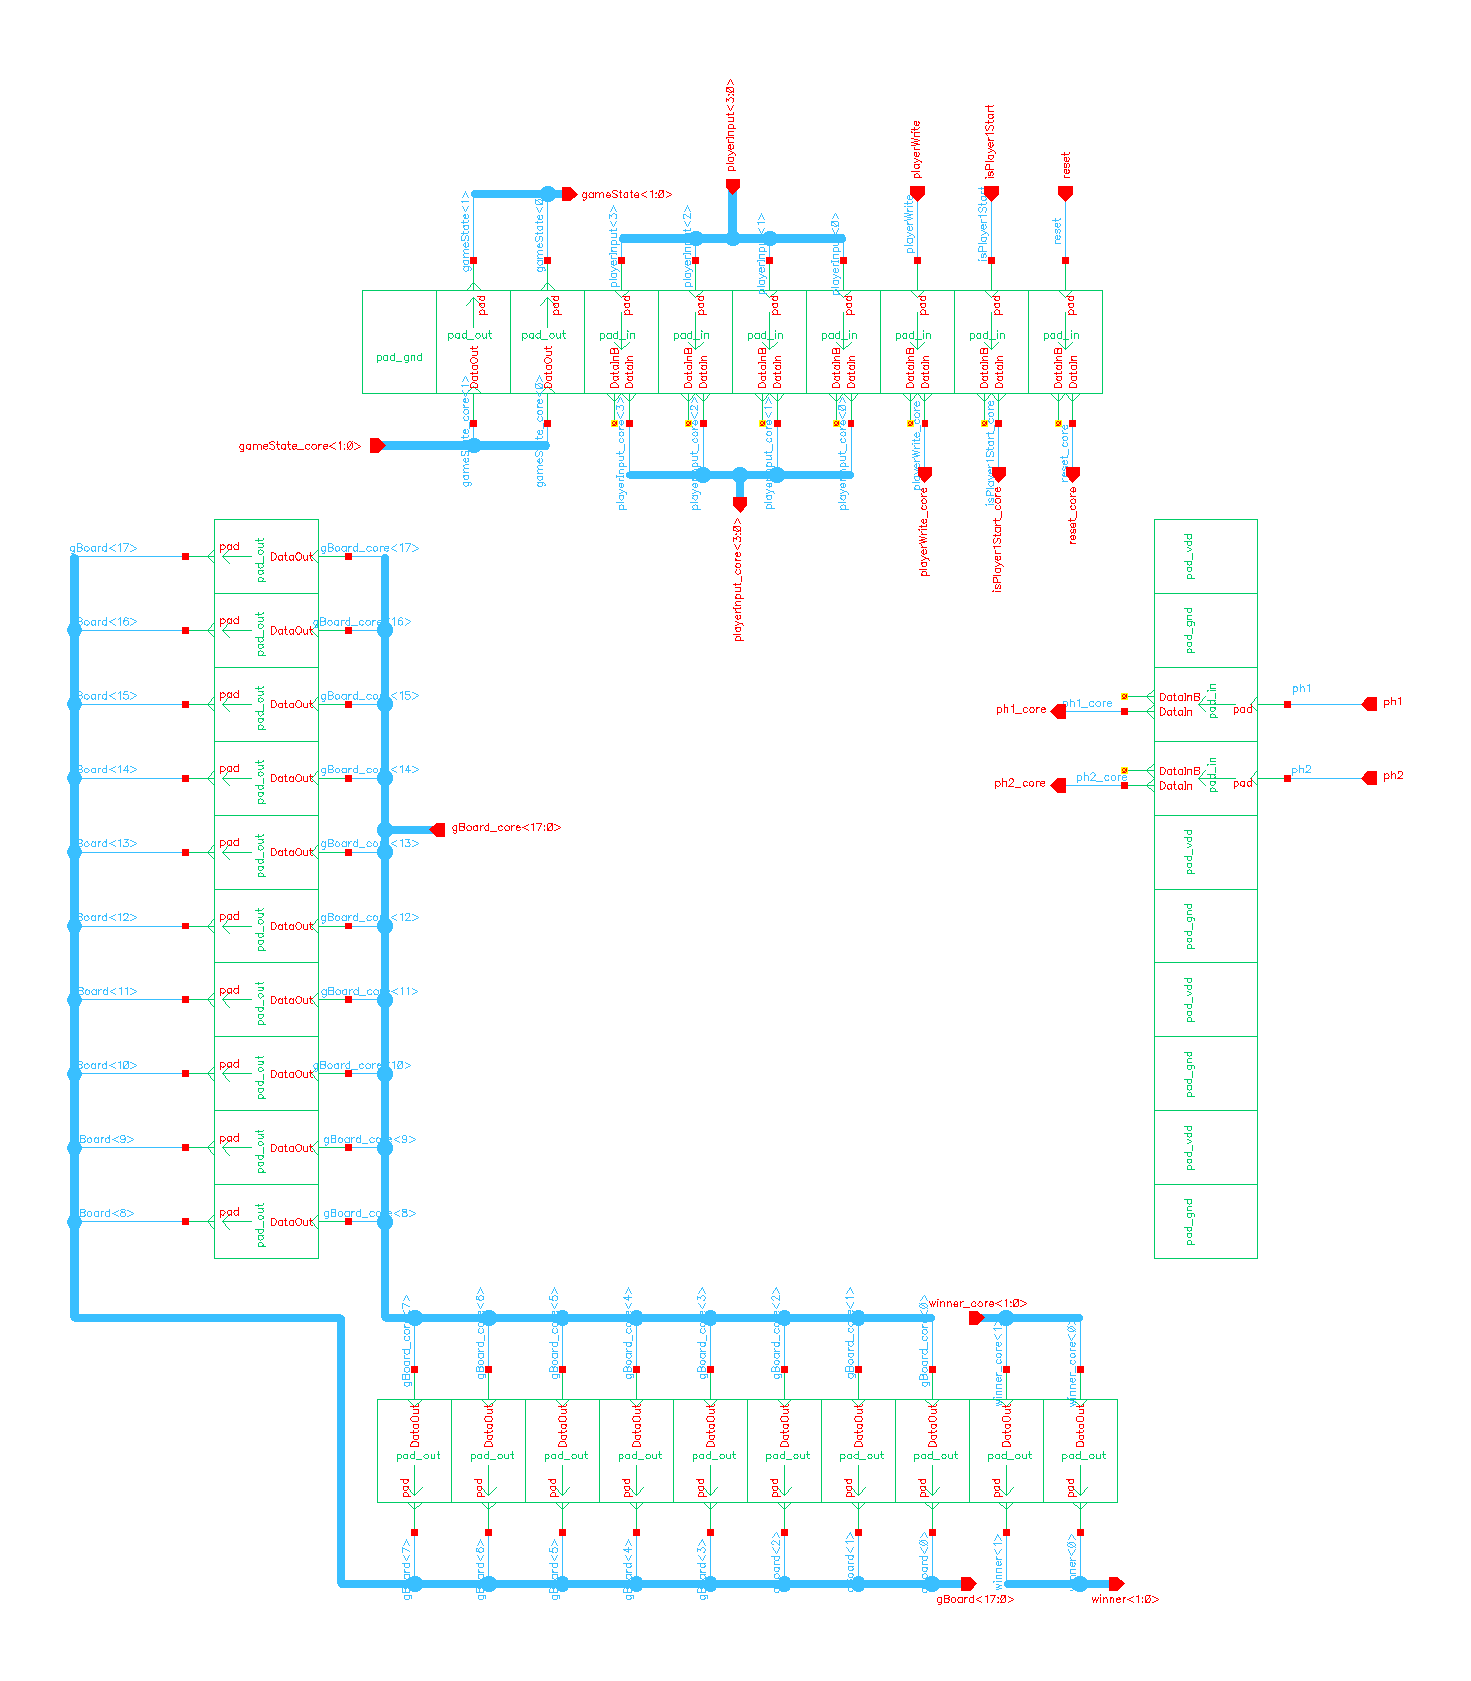
\includegraphics[width=0.9\textwidth]{padframe-schematic}
\caption{Padframe schematic}
\label{fig:padframe-schematic}
\end{figure}

\begin{figure}[H]
\centering
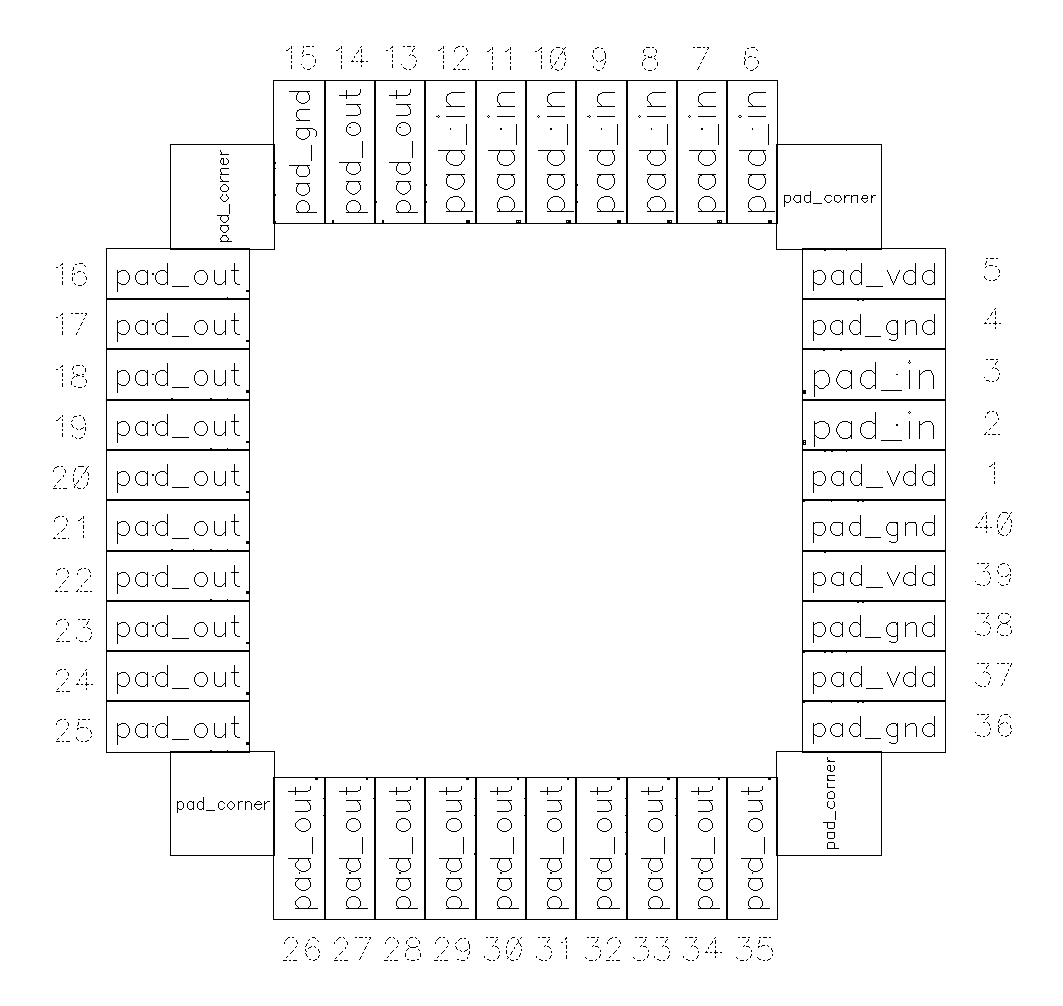
\includegraphics[width=0.9\textwidth]{padframe-layout0}
\caption{Padframe layout}
\label{fig:padframe-layout}
\end{figure}


\subsection{chip}
\begin{figure}[H]
\centering
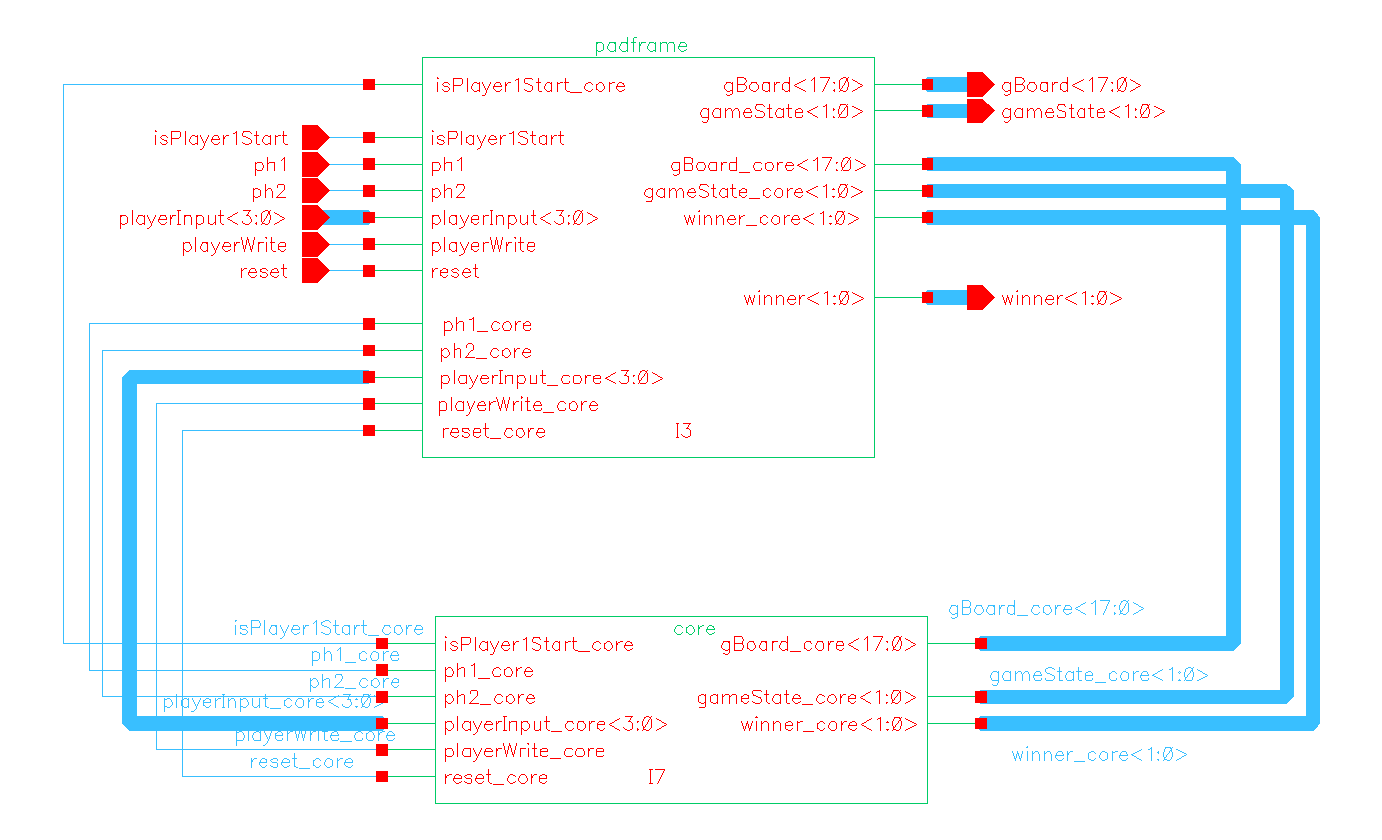
\includegraphics[width=0.9\textwidth]{chip-schematic}
\caption{Chip schematic}
\label{fig:chip-schematic}
\end{figure}

\begin{figure}[H]
\centering
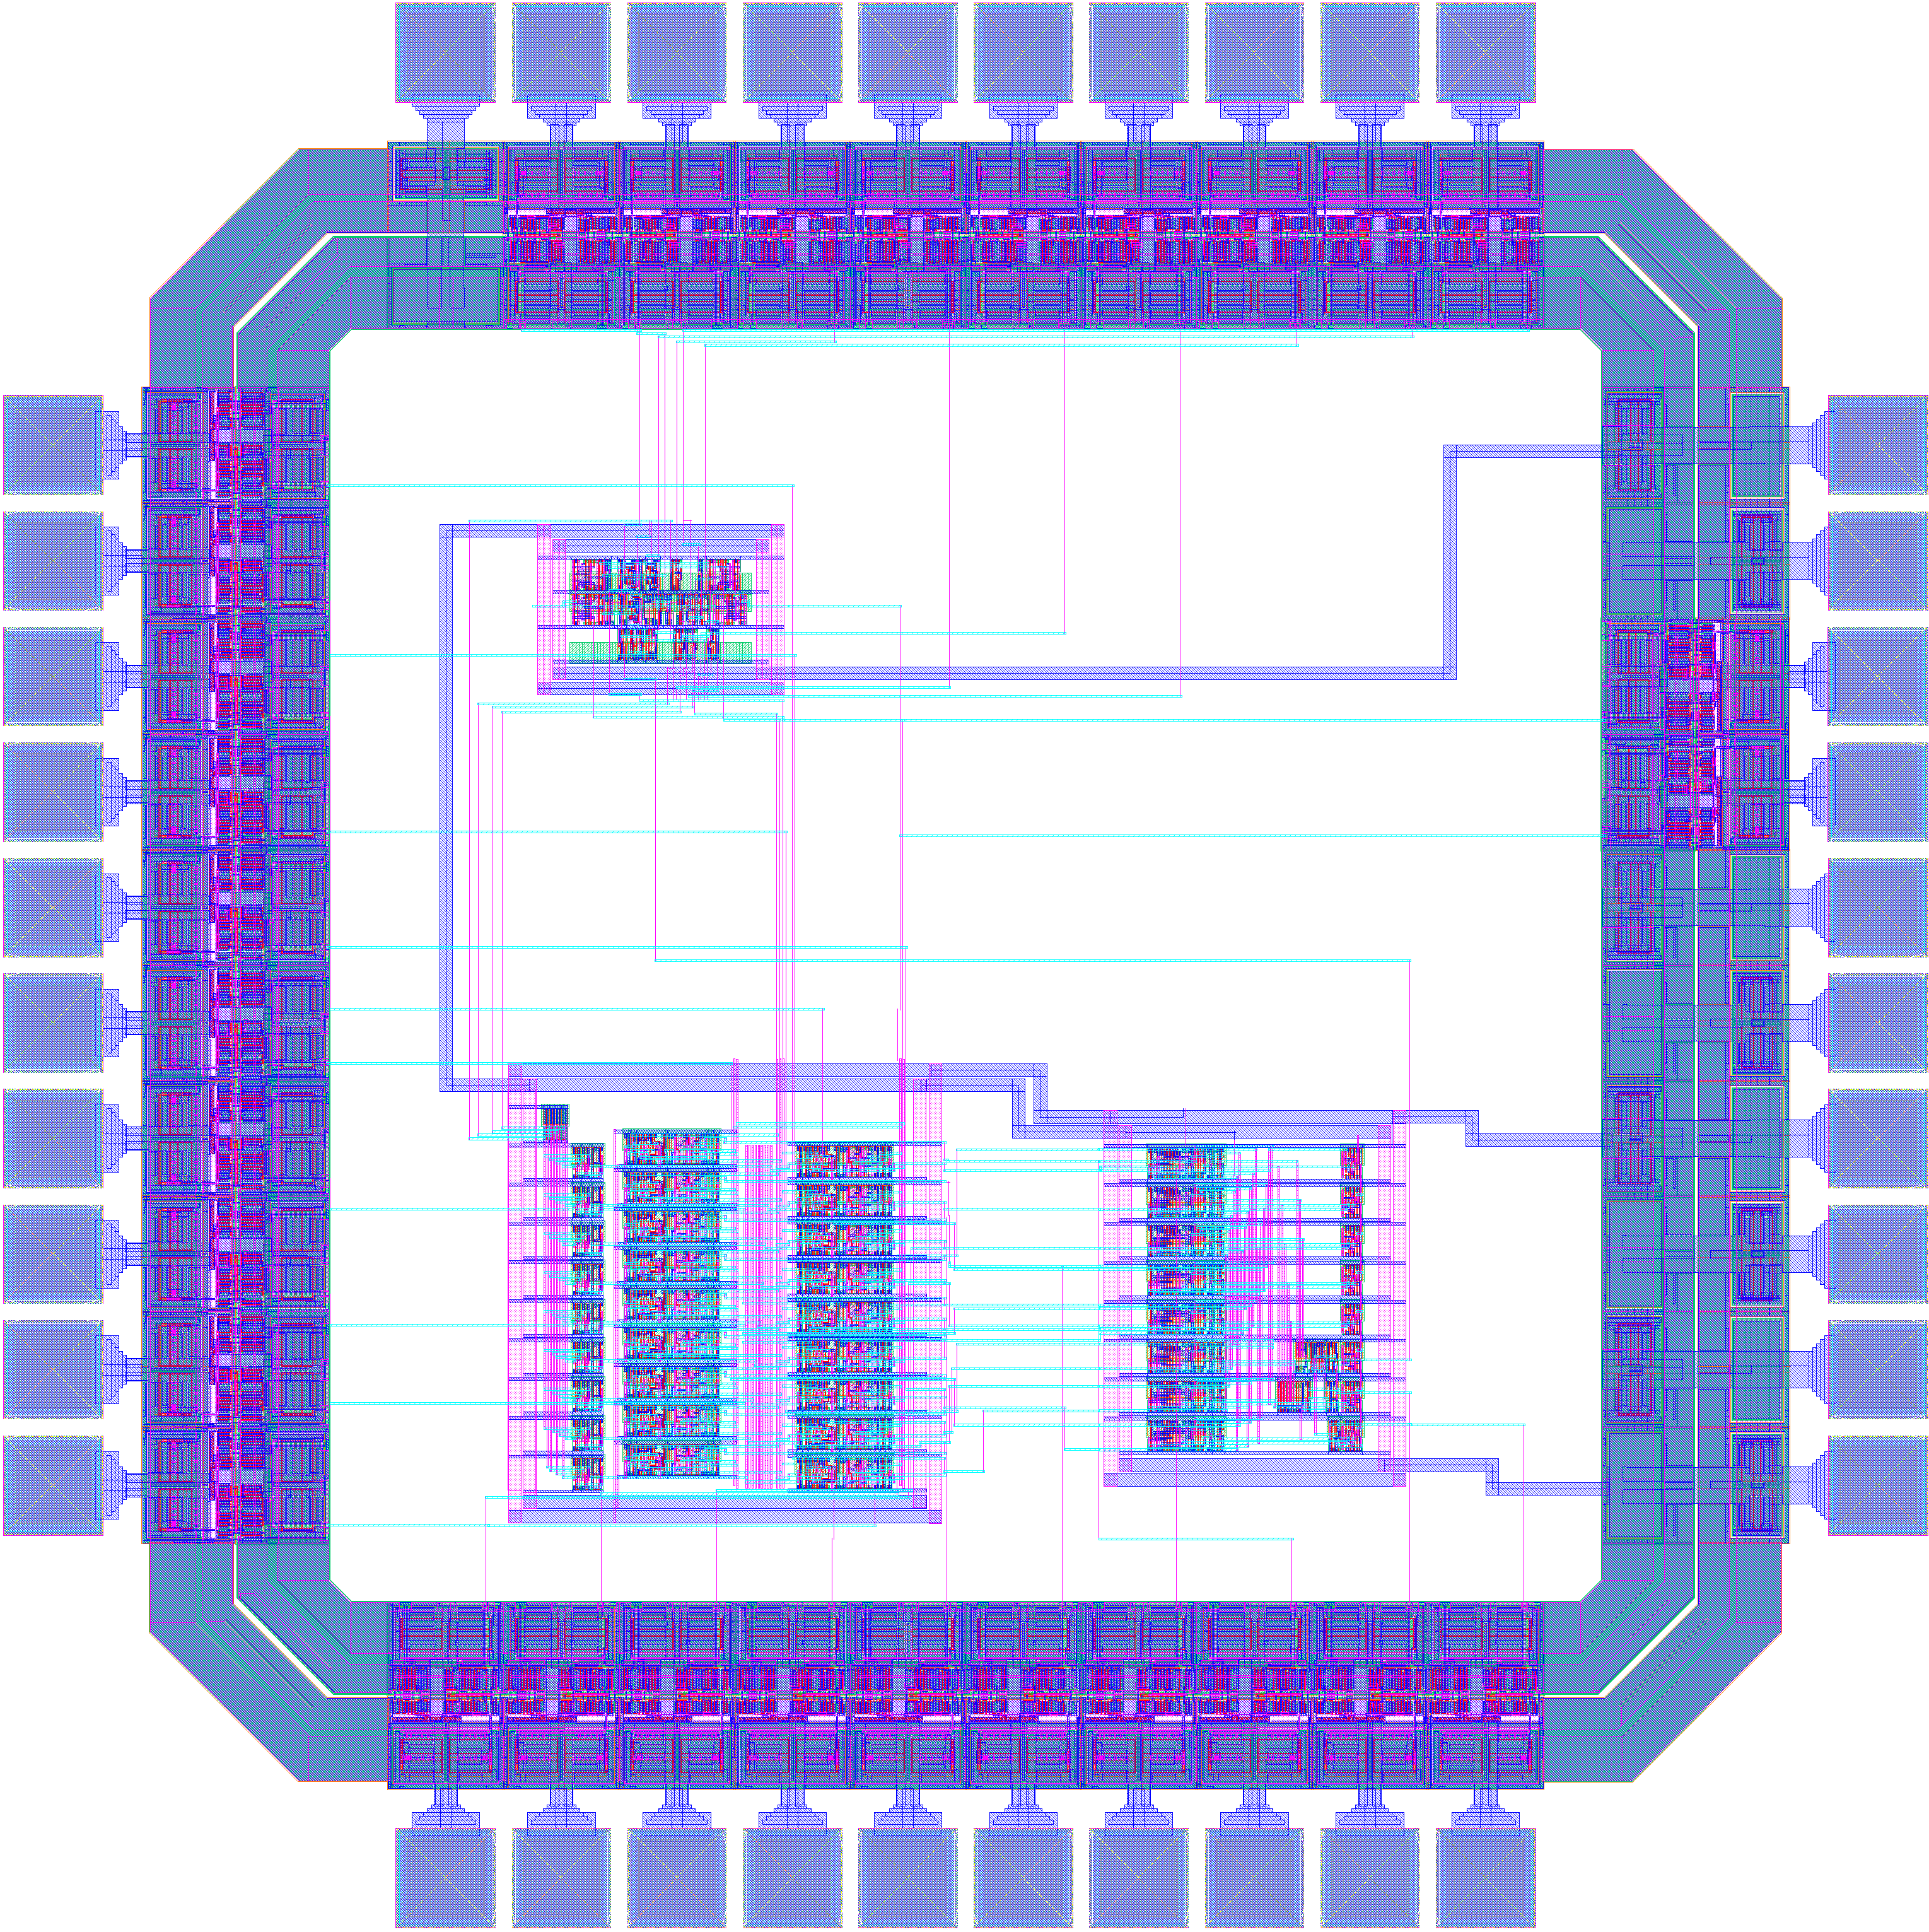
\includegraphics[width=0.9\textwidth]{chip-layout}
\caption{Chip layout}
\label{fig:chip-layout}
\end{figure}


\end{document}
